%==============================================================
%  EZNX-ATLAS-A -- MDPI Mathematics English submission source
%  Version 2.3.3 -- 2026-04-25
%  Numerical cross-check sources bundled in artifacts/statistical_analysis_full.json
%  and artifacts/missingness_eval_demo_anthro_summary.json
%==============================================================
\documentclass[mathematics,article,submit,pdftex]{Definitions/mdpi}

\usepackage{bm}
\providecommand{\history}[1]{}
\providecommand{\TitleCitation}[1]{}
\providecommand{\AuthorCitation}[1]{}
\setlength{\headheight}{20pt}
\AtBeginDocument{%
  \pdfstringdefDisableCommands{%
    \def\textsc#1{#1}%
    \def\texttt#1{#1}%
    \def\mathrm#1{#1}%
    \def\mathbf#1{#1}%
    \def\bm#1{#1}%
    \def\Delta{Delta }%
    \def\pm{plus or minus }%
  }%
  \hypersetup{
    pdftitle={EZNX-ATLAS-A: Measuring the Incremental Contribution of Clinical Metadata to 12-Lead ECG Superclass Classification on PTB-XL},
    pdfauthor={Ezyn SEGNANE, Younes OMMANE, Khalil EL WALED, Mohamedou CHEIKH TOURAD},
    pdfsubject={MDPI Mathematics submission},
    pdfkeywords={electrocardiogram, deep learning, multimodal fusion, missing data, PTB-XL}
  }%
}

% ---- MDPI administrative ----------------------------------
\firstpage{1}
\makeatletter\setcounter{page}{\@firstpage}\makeatother
\pubvolume{1}
\issuenum{1}
\articlenumber{0}
\pubyear{2026}
\copyrightyear{2026}
\datereceived{}
\dateaccepted{}
\datepublished{}
\history{Received: ; Accepted: ; Published: }

% ---- Title and authors -------------------------------------
\Title{EZNX-ATLAS-A: Measuring the Incremental Contribution of Clinical Metadata to 12-Lead ECG Superclass Classification on PTB-XL}
\TitleCitation{EZNX-ATLAS-A: Incremental Metadata Contribution in PTB-XL ECG Classification}

\newcommand{\orcidauthorA}{0009-0005-0538-4335}
\newcommand{\orcidauthorB}{0000-0001-6827-2967}
\newcommand{\orcidauthorC}{0009-0001-7356-032X}
\newcommand{\orcidauthorD}{0000-0003-1273-7512}

\Author{Ezyn~SEGNANE$^{1,\ast}$\orcidA{}, Younes~OMMANE$^{2}$\orcidB{}, Khalil~EL~WALED$^{1}$\orcidC{} and Mohamedou~CHEIKH~TOURAD$^{1}$\orcidD{}}
\AuthorNames{Ezyn SEGNANE, Younes OMMANE, Khalil EL WALED and Mohamedou CHEIKH TOURAD}
\AuthorCitation{SEGNANE, E.; OMMANE, Y.; EL WALED, K.; CHEIKH TOURAD, M.}

\address{%
$^{1}$\quad Faculty of Sciences and Techniques, Al-Khawarizmi, University of Nouakchott, Nouakchott, Mauritania; ezyn.segnane@univ-nkc.mr (E.S.); khalil.elwaled@univ-nkc.mr (K.E.W.); cheikhtouradmohamedou@univ-nkc.mr (M.C.T.)\\
$^{2}$\quad Faculty of Medical Sciences, Mohammed VI Polytechnic University, Ben Guerir, Morocco; Younes.OMMANE@um6p.ma (Y.O.)}
\corres{Correspondence: ezyn.segnane@univ-nkc.mr}

% ---- Abstract ----------------------------------------------
\abstract{We present a paired multi-seed measurement framework for multimodal-ML ablations, applied to ECG combined with clinical metadata on PTB-XL. Effect size, class distribution, and missingness robustness of the metadata signal are rarely quantified under seed-matched protocols. We introduce EZNX-ATLAS-A, a 3.82 million-parameter dual-branch architecture coupling a residual ECG encoder, a demographic and anthropometric encoder, an explicit metadata-availability score, and GLU-style late fusion on PTB-XL 1.0.3. We run a fully crossed ablation of three metadata variants (none, demo, demo+anthro) across 10 random seeds; the full-metadata variant reaches macro-AUC 0.9289 (SD 0.0009). Paired Wilcoxon signed-rank tests with Benjamini--Hochberg correction show that age and sex alone yield no improvement detectable at this protocol's power (Delta = +0.0002, BH-adjusted p = 0.626), consistent with demographics being recoverable from the waveform. Full metadata produce a small but statistically significant gain (Delta macro-AUC = +0.0014, 95 percent paired CI [0.0009, 0.0019], BH-adjusted p = 0.028), concentrated in MI and STTC (ST/T change) rather than in HYP. Under inference-time masking of anthropometric fields, macro-AUC remains within 0.0010 of the unmasked model. These results, conditional on validation-based model selection, provide a reproducibility baseline for multimodal ECG studies, arguing for paired multi-seed statistics, per-class analysis, and explicit missingness audits.}

\keyword{electrocardiogram; multimodal fusion; multiplicative gating; missing data; PTB-XL; myocardial infarction; reproducibility; nonparametric inference}

\MSC{68T07; 68T45; 62P10; 62G10; 92C55}

\begin{document}

% =============================================================
\section{Introduction}\label{sec:intro}
% =============================================================

Automatic interpretation of the 12-lead electrocardiogram is one of the most mature applications of clinical deep learning. Hannun~\textit{et al.}~\cite{Hannun2019} reported cardiologist-level arrhythmia detection on ambulatory single-lead recordings; Ribeiro~\textit{et al.}~\cite{Ribeiro2020} demonstrated large-scale automatic diagnosis from standard 12-lead ECGs; and Attia~\textit{et al.}~\cite{Attia2019LV} showed that a 12-lead CNN could screen for reduced left-ventricular ejection fraction. Siontis~\textit{et al.}~\cite{Siontis2021} review these and related AI-ECG applications in cardiovascular disease management. On the public PTB-XL corpus~\cite{Wagner2020}, the canonical benchmark of Strodthoff~\textit{et al.}~\cite{Strodthoff2021} places superclass macro-AUC at $0.928 \pm 0.005$ for a 1D-ResNet. More recent self-supervised systems~\cite{Mehari2022, Weimann2025, Coppola2024} improve selected ECG benchmarks, but they are waveform-centric and therefore do not directly answer how much structured patient metadata adds to PTB-XL superclass classification.

A natural next step is \emph{multimodal fusion} with structured clinical metadata, since PTB-XL exposes age and sex for nearly all records and height/weight-derived anthropometrics for a smaller subset. Recent ECG-fusion works~\cite{Qiu2024, Srivastava2025, Atwa2025, Holloway2026} show that ECG representations can be combined with clinical variables, patient-characteristic modules, or engineered feature tables. However, our paper-by-paper audit (Tables~\ref{tab:prior_a}--\ref{tab:prior_b}) found that these studies differ in task, dataset, and metadata definition; their reported gains should therefore not be read as direct numerical baselines for PTB-XL superclass demographic/anthropometric fusion. The specific gap we target is narrower: seed-matched ablation of demographics versus anthropometrics, per-class decomposition, and inference-time missingness stress testing.

We contribute a targeted remedy. Rather than proposing yet another ECG backbone, we design \textbf{EZNX-ATLAS-A}---a deliberately compact (3.82\,M parameters) quality-gated dual-branch architecture---and use it as an \emph{instrument} to address four questions. We intentionally keep a compact residual backbone, rather than escalate simultaneously to a larger Transformer or foundation waveform encoder, so that measured gains are easier to attribute to the metadata pathway itself and so that 30 seed-matched runs remain computationally tractable:

\begin{description}[leftmargin=1.5em, style=sameline, font=\bfseries]
\item[Q1.] When, if ever, does structured clinical metadata meaningfully improve PTB-XL superclass classification, once seed variance is accounted for?
\item[Q2.] Which \emph{type} of metadata (demographic vs.\ anthropometric) helps which pathology class?
\item[Q3.] Can a quality-gated fusion degrade gracefully as anthropometric metadata fields are withheld, remaining near the ECG-only and demographics-only baselines?
\item[Q4.] How do our measured effects compare with recent multimodal ECG reports once task, dataset, metadata definition, and statistical protocol are audited?
\end{description}

Our answers, detailed in Sections~\ref{sec:results}--\ref{sec:discussion}, challenge some intuitions: (Q1) demographics alone ($\texttt{demo}$ minus $\texttt{none}$) yield no improvement detectable at this protocol's power ($\Delta{=}{+}0.0002$ macro-AUC, 95\% paired seed-level CI $[-0.0002, 0.0007]$, $p_{\mathrm{BH}}{=}0.626$), consistent with the known recoverability of age and sex from the raw 12-lead waveform~\cite{Attia2019AgeSex}. Anthropometrics add a small but statistically significant gain beyond demographics ($\Delta{=}{+}0.0012$ macro-AUC, 95\% paired seed-level CI $[0.0007, 0.0018]$, $p_{\mathrm{BH}}{=}0.028$); (Q2) the full-metadata gain over ECG alone concentrates in the \emph{MI} and \emph{STTC} superclasses, while HYP does not show the strong effect suggested by voltage-based LVH criteria---an apparent puzzle that we revisit as a hypothesis in Section~\ref{sec:discussion}; (Q3) yes, with macro-AUC loss $\approx 0.0010$ under full anthropometric dropout at inference; (Q4) the audited literature motivates multimodal fusion but does not provide a directly comparable seed-matched PTB-XL demographic/anthropometric baseline. We therefore position this paper as a cautious measurement study that replaces a broad multimodal claim with a statistically honest, class-localised one.

Beyond the ECG application, this paper introduces a reusable statistical measurement pipeline for multimodal-ML ablations: exact two-sided paired Wilcoxon signed-rank tests on seed-matched differences, Benjamini--Hochberg FDR control at $q{=}0.05$ across a pre-declared 36-test pre-specified family, and percentile bootstrap CIs for paired differences. This pipeline, formalised in Section~\ref{sec:protocol}, applies to any ablation study in which model variants are compared across repeated random seeds.

% =============================================================
\section{Related Work}\label{sec:relwork}
% =============================================================

\subsection{Supervised benchmarks on PTB-XL}
Wagner~\textit{et al.}~\cite{Wagner2020} released PTB-XL, a 21\,799-record 12-lead corpus with SCP-ECG multi-label annotations aggregated into 5 superclasses, 23 sub-classes and 44 diagnostic statements, together with a stratified, patient-disjoint 10-fold partition. Strodthoff~\textit{et al.}~\cite{Strodthoff2021} established the canonical benchmark, reporting macro-AUC $0.928(5)$ on super-diag with xresnet1d101. Nonaka and Seita~\cite{Nonaka2021} swept nine 1D-CNN backbones and found ResNet-18 competitive with deeper variants. The Bydgoszcz group~\cite{Smigiel2021, Palczynski2022} studied entropy features and few-shot learning but used a non-standard 70/15/15 split, making their numbers incomparable to the canonical benchmark. In the supervised PTB-XL benchmark papers audited here, we did not identify a seed-matched age/sex vs.\ anthropometric ablation with an explicit missing-metadata stress test.

\subsection{Landmark clinical ECG models}
Hannun~\textit{et al.}~\cite{Hannun2019} reached cardiologist-level rhythm classification on 91\,232 single-lead ambulatory ECGs; Ribeiro~\textit{et al.}~\cite{Ribeiro2020} generalised to 12-lead short recordings on a 2M-record Brazilian telehealth corpus. Attia~\textit{et al.}~\cite{Attia2019LV} showed a CNN could screen for LV ejection fraction $\leq 35\%$ directly from the 12-lead ECG (AUC 0.93). Critically for the present paper, Attia~\textit{et al.}~\cite{Attia2019AgeSex} demonstrated that age and sex are themselves \emph{recoverable} from the raw ECG (age MAE 6.9\,y, sex AUC 0.97), supporting the idea that demographic signal is already partly present in the waveform. Siontis~\textit{et al.}~\cite{Siontis2021} identify this latent-demographic phenomenon as both an opportunity and a confounding risk.

\subsection{Self-supervised and foundation ECG models}
Contrastive and masked-modelling approaches---CLOCS~\cite{Kiyasseh2021}, CPC-based pretraining~\cite{Mehari2022}, ST-MEM~\cite{Na2024}, the ECG joint-embedding predictive architecture (ECG-JEPA)~\cite{Weimann2025}, and preprint waveform foundation models such as HuBERT-ECG~\cite{Coppola2024} and TolerantECG~\cite{Nguyen2025}---study representation learning and robustness from waveform inputs alone, including PTB-XL downstream evaluations in some cases. They are therefore adjacent to, but distinct from, the metadata-value question studied here. The non-peer-reviewed preprints in this paragraph are cited as contextual neighbouring work rather than as pre-specified baselines.

\subsection{Multimodal ECG + tabular fusion}
Explicit ECG + tabular or feature-fusion architectures have begun to appear, but they are not interchangeable baselines. Qiu~\textit{et al.}~\cite{Qiu2024} fuse a transformer ECG encoder with clinical features for atrial-fibrillation recurrence prediction after ablation, outside PTB-XL. The preprint rECGnition\_v2.0 system~\cite{Srivastava2025} studies self-attentive canonical fusion on MIT-BIH, INCARTDB and the European ST-T Database. Among PTB-XL-family studies, Atwa~\textit{et al.}~\cite{Atwa2025} (whose published title uses the abbreviation ``PTB-X'', referring to the same PhysioNet corpus) is the closest published demographic-fusion comparator because it adds age and sex to CNN/VGG-style arrhythmia models; however, it reports accuracy-oriented results across 2-, 5-, 10-, and 15-class tasks with augmentation rather than seed-matched macro-AUC on the canonical five-superclass split. In parallel, PTB-XL+~\cite{Strodthoff2023PTBXLPlus} augments PTB-XL with engineered Uni-G, 12SL and ECGDeli feature tables; Holloway~\textit{et al.}~\cite{Holloway2026} compare raw PTB-XL signals with such PTB-XL+ feature representations. These feature tables are derived from the ECG itself rather than from EHR-like anthropometrics. We therefore treat these papers as motivation and methodological context, not as direct numerical comparators; the exact comparability audit is summarised in Tables~\ref{tab:prior_a}--\ref{tab:prior_b}.

\subsection{Gated fusion mechanisms}
The Gated Linear Unit (GLU) of Dauphin~\textit{et al.}~\cite{Dauphin2017} provides a simple multiplicative gate $\mathbf{h} \odot \sigma(\cdot)$ that preserves linear gradient flow. The Gated Multimodal Unit~\cite{Arevalo2020} extends this to modality-level mixing. In medical imaging, Chen~\textit{et al.}~\cite{Chen2019MICCAI} use feature disentanglement plus gated fusion for brain-tumor segmentation, and Kim~\textit{et al.}~\cite{Kim2018ACCV} introduce reliability-aware gates for sensor dropout. We use a GLU-based gate conditioned on an explicit scalar quality score $q_{\mathrm{meta}}$ derived from the metadata-availability mask.

\subsection{Missing modalities in clinical ML}
Baltru{\v{s}}aitis~\textit{et al.}~\cite{Baltrusaitis2019} survey the main settings of multimodal learning, including fusion and co-learning under incomplete modalities. HeMIS~\cite{Havaei2016}, SMIL~\cite{Ma2021}, and mmFormer~\cite{Zhang2022} address missing modalities in imaging or general multimodal settings rather than ECG+tabular fusion. We study the adjacent ECG+tabular setting by coupling an availability-mask-driven quality score with stochastic sample meta-dropout during training.

\subsection{Clinical motivation for anthropometrics in ECG classification}
Classical ECG LVH criteria---Sokolow--Lyon~\cite{Sokolow1949}, Cornell voltage/duration product~\cite{Casale1985}, Romhilt--Estes~\cite{Romhilt1968}, and Peguero--Lo Presti~\cite{Peguero2017}---depend on measured voltage and are affected by body habitus. Left ventricular mass is itself routinely indexed to body surface area or $\mathrm{height}^{2.7}$. \emph{A priori}, these cardiology facts suggest that the HYP superclass could benefit from anthropometric metadata. More broadly, ECG amplitudes and repolarisation measurements relevant to MI and STTC can also be influenced by torso conduction properties, lead geometry, and recording context~\cite{Rautaharju2009, MacFarlane2011}, suggesting possible relevance of body-size priors across morphology-rich classes. Our per-class results in Section~\ref{sec:results} are compatible with this broader relevance while not supporting a strong HYP-specific effect at the superclass level.

% =============================================================
\section{Dataset and Preprocessing}\label{sec:dataset}
% =============================================================

\subsection{PTB-XL 1.0.3}
We use PTB-XL version 1.0.3 on PhysioNet~\cite{Wagner2020,Goldberger2000} at 100\,Hz sampling rate ($T{=}1000$ samples, 10\,s, 12 leads). Following~\cite{Strodthoff2021}, SCP-ECG diagnostic statements are mapped to the 5-class super-diagnostic task $\{\mathrm{NORM}, \mathrm{MI}, \mathrm{STTC}, \mathrm{CD}, \mathrm{HYP}\}$ using \path{scp_statements.csv}. In the implemented loader, a record is positive for a superclass if any diagnostic SCP code assigned to that class is present in \path{scp_codes}; no additional likelihood threshold is applied at load time. The official stratified-by-label and patient-disjoint 10-fold partition is used unchanged in the working index: folds 1--8 for training, fold 9 for validation, fold-10 for test, yielding 17{,}418 / 2{,}183 / 2{,}198 records, respectively (Table~\ref{tab:dataset}). These fold counts sum to 21\,799 records, matching the current PhysioNet v1.0.3 release after the duplicate removals documented in its release notes. A package-local integrity report additionally verifies zero shared patient IDs across the train/validation/test partitions of the working index.

\subsection{Formal multi-label problem setting}
For each record $i$, the loader returns a quadruple
\[
(\mathbf{X}_i,\mathbf{x}_i,\mathbf{m}_i,\mathbf{y}_i)
\in \mathbb{R}^{12\times1000}\times\mathbb{R}^{8}\times\{0,1\}^{8}\times\{0,1\}^{5},
\]
where $\mathbf{X}_i$ is the ECG, $\mathbf{x}_i$ is the imputed metadata vector, $\mathbf{m}_i$ is its availability mask, and $\mathbf{y}_i$ is the multi-hot superclass target. A model with parameters $\theta$ emits logits $\bm{\ell}_{i}(\theta)\in\mathbb{R}^{5}$ and probabilities $\mathbf{p}_{i}=\sigma(\bm{\ell}_{i})$. The principal metric is
\[
\mathrm{macroAUC}(\theta)=\frac{1}{5}\sum_{c=1}^{5}\mathrm{AUC}\bigl(\{(y_{ic},p_{ic})\}_{i\in\mathcal{D}_{\mathrm{test}}}\bigr),
\]
with class-wise AUC skipped only if a class is degenerate, which does not occur for the PTB-XL superclasses on fold-10. The ablations below are deterministic interventions on $(\mathbf{x}_i,\mathbf{m}_i)$, so seed-matched comparisons estimate the incremental contribution of metadata while holding the architecture, optimiser, folds, and random seed fixed.

\subsection{Metadata extraction and normalisation}
From the PTB-XL metadata we construct the 8-dimensional tabular vector
\begin{equation}\label{eq:xmeta}
\mathbf{x}_{\mathrm{meta}}
= \bigl[\underbrace{\mathrm{age}_z,\ \mathrm{sex01}}_{\text{demographic}},\ 
         \underbrace{\mathrm{height}_z,\ \mathrm{weight}_z,\ \mathrm{bmi}_z}_{\text{anthropometric}},\ 
         \underbrace{m_h,\ m_w,\ m_{\mathrm{bmi}}}_{\text{missingness indicators}}\bigr]
\in \mathbb{R}^{8},
\end{equation}
where $\mathrm{sex01}\in\{0,1\}$, subscript $z$ denotes standardisation using training-fold mean and standard deviation after median imputation, BMI is derived from height and weight when both are observed and otherwise imputed, and $m_{\cdot}\in\{0,1\}$ flags whether each anthropometric field was missing before imputation. The availability mask $\mathbf{m}\in\{0,1\}^{8}$ follows the implemented index columns \texttt{mask\_\_*}. For the three missingness-indicator channels, \texttt{mask\_\_miss\_*} is tied to the corresponding original anthropometric field, so unavailable height, weight, or BMI both sets the indicator value to 1 and lowers the quality score through a zero mask bit. Put differently, the \texttt{miss\_\_*} values live inside $\mathbf{x}_{\mathrm{meta}}$ to tell the model which anthropometric slot was imputed, whereas the \texttt{mask\_\_*} bits in $\mathbf{m}$ drive availability-aware scaling; the two channels are therefore intentionally complementary rather than accidental duplicates. In the working index, sex is always observed, age is observed for 98.7\% of records, and anthropometric availability is substantially lower (Table~\ref{tab:dataset}).

\subsection{Positive class weights from training-set prevalence}
Let $f_c$ denote the training-fold prevalence of each superclass. We derive the binary cross-entropy positive weights by normalising the positive-class inverse odds to NORM:
\begin{equation}\label{eq:posweights}
w_c^{+} \;=\; \frac{(1-f_c)/f_c}{(1-f_{\mathrm{NORM}})/f_{\mathrm{NORM}}}, \qquad c\in\{\mathrm{NORM},\mathrm{MI},\mathrm{STTC},\mathrm{CD},\mathrm{HYP}\}.
\end{equation}
Normalising to NORM anchors the weight vector to the most-prevalent class (training prevalence 43.6\%), yielding relative weights that grow with class rarity while keeping the NORM weight at unity; this avoids a globally inflated loss scale and makes the weight vector interpretable as a rarity ratio relative to the reference class. Computed on the training folds 1--8 of PTB-XL~1.0.3, this yields the fixed weight vector reported in Table~\ref{tab:dataset}. This weighting is a \emph{loss-level} re-scaling applied per positive label inside the binary cross-entropy; it does \emph{not} alter the class distribution at the data level (no oversampling, undersampling, or label replication is performed). This weighting is derived from the training-fold class frequencies via Eq.~\eqref{eq:posweights}: the resulting weight vector $[w_{\mathrm{NORM}}^+, w_{\mathrm{MI}}^+, w_{\mathrm{STTC}}^+, w_{\mathrm{CD}}^+, w_{\mathrm{HYP}}^+] = [1.0,\ 2.3,\ 2.44,\ 2.67,\ 5.58]$ was computed once on folds~1--8 and held fixed across all 30 runs to ensure exact reproducibility; the values are fully determined by the public PTB-XL statistics and thus reproducible without access to any private signal.

\subsection{Preprocessing}
Signals are loaded with \texttt{wfdb} at 100\,Hz, padded or truncated to 1000 time samples, transposed to channel-first shape $(12,T)$, cast to \texttt{float32}, and divided by 5.0 before entering the model. This fixed divisor acts as a conservative millivolt-scale preconditioner that keeps typical 12-lead amplitudes near unit scale without introducing fold-specific waveform z-normalisation. Before imputation, out-of-range metadata are converted to missing using conservative physiological bounds: age 0--120 years, height 120--210\,cm, weight 30--250\,kg, and BMI 10--60. These BMI bounds are intentionally broad: they function as a sanity screen for grossly implausible entries rather than as a clinical trimming rule, and records are retained because only the affected metadata fields are masked and imputed. Evaluation splits (validation and test) apply only the fixed divisor; training additionally uses light stochastic augmentation. The augmentation block fires with probability 0.5 per training mini-batch. Inside it, three operations each trigger independently at probability 0.3: additive Gaussian noise ($\sigma{=}0.02$, with sample-specific noise draws), a random integer temporal shift (uniform on $[-20,+19]$ samples, shared across the mini-batch), and a multiplicative amplitude jitter whose factor is drawn uniformly from $[0.95, 1.05]$ (shared across the mini-batch). These hyperparameters were set to conservative values before the seed sweep and were not ablated; this is a deliberate choice to avoid multiplying the compute budget, and they are reported here for full reproducibility. Labels are multi-hot vectors of length 5, one entry per superclass.

% =============================================================
\section{Model Architecture: EZNX-ATLAS-A}\label{sec:model}
% =============================================================

Figure~\ref{fig:arch} shows the complete architecture. We describe each block with its dimensional signature and design rationale.

\begin{figure}[H]
\centering

\includegraphics[width=\linewidth]{figures/fig1_architecture.pdf}
\caption{\textbf{EZNX-ATLAS-A architecture.} The 1D residual ECG backbone emits a 1024-dim temporal-statistics embedding $\mathbf{h}_{\mathrm{ts1}}$. A dual demographic/anthropometric MLP stack produces $\mathbf{h}_{\mathrm{m}}\in\mathbb{R}^{128}$, scaled by an explicit availability score $q_{\mathrm{meta}}$. A residual injection with a zero-initialised $1024\times 128$ projection softly biases the ECG embedding, and a GLU-style multiplicative gate fuses the concatenated embeddings. Three classification heads (fused, ECG-only, meta-only) enable multi-loss training; inference uses a validation-tuned convex blend of fused and ECG-only probabilities. The gate itself contains 2.66\,M of the 3.82\,M trainable parameters (69.5\%), while the metadata-to-ECG residual projection adds 0.13\,M (3.4\%). Table~\ref{tab:hparams} reports the matched parameter budget and the archived compute provenance.}
\label{fig:arch}
\end{figure}

\subsection{ECG branch: TSBackbone1D\_v5}
An initial Conv1D ($k{=}7$, $s{=}2$, $p{=}3$, $12{\to}64$) with BatchNorm and ReLU is followed by MaxPool ($k{=}3$, $s{=}2$, $p{=}1$). Three residual stages, each with two residual blocks, implement the channel schedule $64{\to}64$ (stride 1), $64{\to}128$ (stride 2), $128{\to}256$ (stride 2), giving an output of shape $256\times T'$ with $T'{=}63$ for $T{=}1000$. A \emph{Temporal Statistics Pool} concatenates mean, standard deviation, max, and min over time:
\begin{equation}
\mathbf{h}_{\mathrm{ts1}}
= \bigl[\,\mu(\mathbf{F}),\ \sigma(\mathbf{F}),\ \max(\mathbf{F}),\ \min(\mathbf{F})\,\bigr]
\in \mathbb{R}^{1024}, \qquad \mathbf{F}\in\mathbb{R}^{256\times T'}.
\end{equation}
The four-moment pool captures both aggregate waveform energy and extreme amplitudes, which are diagnostic for MI (ST deviation, Q-wave depth) and HYP (voltage maxima).

\subsection{Dual metadata encoder}
The loader returns the 8-dim tabular vector in Eq.~\eqref{eq:xmeta} together with its 8-dim availability mask. The model therefore forms a 4-dim demographic slice (age and sex plus their two availability bits) and a 12-dim anthropometric slice obtained by concatenating the six anthropometric values/indicators with their six availability bits:
\begin{align}
\mathbf{h}_{\mathrm{demo}}   &= \mathrm{MLP}_{\mathrm{demo}}(\mathbf{x}_{\mathrm{demo}}):\ \mathbb{R}^{4}\to\mathbb{R}^{64}\to\mathbb{R}^{64}\to\mathbb{R}^{64}, \\
\mathbf{h}_{\mathrm{anthro}} &= \mathrm{MLP}_{\mathrm{anthro}}(\mathbf{x}_{\mathrm{anthro}}):\ \mathbb{R}^{12}\to\mathbb{R}^{96}\to\mathbb{R}^{96}\to\mathbb{R}^{64}.
\end{align}
Each intermediate linear layer uses ReLU, BatchNorm, and 10\% Dropout; the final linear layer uses ReLU only.

\subsection{Availability-aware quality score}
We define per-block availability scores and an aggregate metadata-quality score:
\begin{equation}\label{eq:qmeta}
q_{d} = \tfrac{1}{2}\sum_{i=0}^{1} m_i, \qquad
q_{a} = \tfrac{1}{6}\sum_{i=2}^{7} m_i, \qquad
q_{\mathrm{meta}} = \min\!\bigl(1,\ q_{d} + 0.5\,q_{a}\bigr).
\end{equation}
In the working index, sex is always observed and age is observed for 98.7\% of records, so $q_d$ is usually 1 and can drop to 0.5 when age is missing. The coefficient 0.5 in front of $q_a$ is a deliberate block-level weighting: demographics define the base availability score, while anthropometrics act as a bounded booster rather than allowing six anthropometric mask slots to outweigh the two demographic slots. The aggregate score $q_{\mathrm{meta}}$ therefore rescales the metadata contribution according to both demographic and anthropometric availability.
In the bundled working-index audit, $q_{\mathrm{meta}}{=}1.0$ for 99.34\% of records, $q_{\mathrm{meta}}{=}0.50$ for 0.60\%, and $q_{\mathrm{meta}}{=}0.6667$ for 0.055\%. The conservative $q_{\mathrm{meta}}^2$ attenuation discussed below therefore acts almost entirely on the rare incomplete-metadata cases rather than on the bulk of the cohort.

\subsection{Meta-fusion MLP with sample meta-dropout}
Concatenation of the encoder outputs with the two availability scalars produces (where $\Vert$ denotes vector concatenation)
\begin{equation}
\begin{aligned}
\widetilde{\mathbf{h}}_{\mathrm{anthro}} &= q_a\,\mathbf{h}_{\mathrm{anthro}},\\
\mathbf{u}_{\mathrm{m}}&=[\mathbf{h}_{\mathrm{demo}}\Vert\widetilde{\mathbf{h}}_{\mathrm{anthro}}\Vert q_d\Vert q_a]\in\mathbb{R}^{130},\\
\bar{\mathbf{h}}_{\mathrm{m}}&=\mathrm{MLP}_{\mathrm{m}}(\mathbf{u}_{\mathrm{m}})\in\mathbb{R}^{128},\qquad
\mathbf{h}_{\mathrm{m}}=q_{\mathrm{meta}}\,\bar{\mathbf{h}}_{\mathrm{m}}.
\end{aligned}
\end{equation}
Thus the anthropometric encoder output is attenuated before meta-fusion when anthropometric availability is low, and the scalar $q_a$ is also exposed explicitly to the meta-fusion MLP. The exact implemented order is Linear$(130,128)$, ReLU, BatchNorm, Dropout$(0.10)$, Linear$(128,128)$, ReLU. During training with probability $p{=}0.10$, the entire pre-quality embedding $\bar{\mathbf{h}}_{\mathrm{m}}$ is zeroed for the sample (\emph{sample meta-dropout}); the quality-scaled embedding $\mathbf{h}_{\mathrm{m}}=q_{\mathrm{meta}}\bar{\mathbf{h}}_{\mathrm{m}}$ is then used by the downstream heads. At inference the sample meta-dropout is disabled and the same $q_{\mathrm{meta}}$ scaling is applied. This design encourages graceful degradation when the metadata embedding is dropped during training or anthropometric fields are withheld at inference.

\subsection{Residual injection}
To prevent the metadata pathway from perturbing ECG representations early in training, we inject a zero-initialised, small-gain residual from $\mathbf{h}_{\mathrm{m}}$ into $\mathbf{h}_{\mathrm{ts1}}$:
\begin{equation}\label{eq:hts}
\mathbf{h}_{\mathrm{ts}} \;=\; \mathbf{h}_{\mathrm{ts1}} + 0.10\cdot q_{\mathrm{meta}}\,\mathbf{W}_{\mathrm{res}}\,\mathbf{h}_{\mathrm{m}},
\qquad \mathbf{W}_{\mathrm{res}}\in\mathbb{R}^{1024\times 128},\ \mathbf{W}_{\mathrm{res}}\!\leftarrow\!0 \text{ at init.}
\end{equation}
The factor $0.10$ and zero initialisation make this residual-injection path neutral at initialisation. Because $\mathbf{h}_{\mathrm{m}}$ is already quality-scaled, the implemented residual path is additionally attenuated by $q_{\mathrm{meta}}$, yielding an effective $q_{\mathrm{meta}}^{2}$ attenuation under partial metadata. We treat this as a deliberate conservative design choice rather than as an accidental duplication: the residual path is the most intrusive metadata-to-ECG route, so it is the one we attenuate most aggressively. Metadata can still enter the fused head through the concatenated representation and the small meta-correction term below. The coefficients 0.10 here and 0.05 in Eq.~\eqref{eq:headfused} were fixed as small-gain stabilisers before the seed sweep; they were not tuned post hoc on the test fold.

\subsection{GLU-style fusion gate}
The fused representation is
\begin{equation}
\mathbf{h} = [\mathbf{h}_{\mathrm{ts}}\Vert \mathbf{h}_{\mathrm{m}}]\in\mathbb{R}^{1152}, \qquad
\mathbf{z} = \mathbf{h} \odot \sigma\!\bigl(\mathrm{Linear}_2(\mathrm{ReLU}(\mathrm{Linear}_1(\mathbf{h})))\bigr)\in\mathbb{R}^{1152},
\end{equation}
where $\mathrm{Linear}_1,\mathrm{Linear}_2:\mathbb{R}^{1152}\to\mathbb{R}^{1152}$, $\odot$ denotes the element-wise (Hadamard) product, and $\sigma(\cdot)$ here denotes the sigmoid activation function. This GLU-style multiplicative gate~\cite{Dauphin2017} lets the model selectively attenuate or preserve individual feature dimensions independently of their modality of origin.

\subsection{Three heads with meta-correction}
Three linear heads produce logits:
\begin{align}
\bm{\ell}_{\mathrm{ecg}}   &= \mathbf{W}_{\mathrm{ecg}}\,\mathbf{h}_{\mathrm{ts1}} + \mathbf{b}_{\mathrm{ecg}}, &\mathbf{W}_{\mathrm{ecg}}\in\mathbb{R}^{5\times 1024}, \\
\bm{\ell}_{\mathrm{meta}}  &= \mathbf{W}_{\mathrm{meta}}\,\mathbf{h}_{\mathrm{m}} + \mathbf{b}_{\mathrm{meta}}, &\mathbf{W}_{\mathrm{meta}}\in\mathbb{R}^{5\times 128}, \\
\bm{\ell}_{\mathrm{fused}} &= \mathbf{W}_{\mathrm{fused}}\,\mathbf{z} + \mathbf{b}_{\mathrm{fused}} + 0.05\,q_{\mathrm{meta}}\,\bm{\ell}_{\mathrm{meta}}, &\mathbf{W}_{\mathrm{fused}}\in\mathbb{R}^{5\times 1152}. \label{eq:headfused}
\end{align}
Critically, $\bm{\ell}_{\mathrm{ecg}}$ is computed on $\mathbf{h}_{\mathrm{ts1}}$ \emph{before} the residual injection in Eq.~\eqref{eq:hts}, preserving a strictly unimodal ECG branch for inference-time blending and ablation. The small additive meta-correction in Eq.~\eqref{eq:headfused} uses the pre-sigmoid metadata logits $\bm{\ell}_{\mathrm{meta}}$, giving the metadata a second, explicit path that bypasses the GLU.

\subsection{Parameter budget}
The total is 3.82\,M trainable parameters: 0.96\,M in the ECG backbone, 0.06\,M in the dual metadata encoders and metadata-fusion MLP, 2.66\,M in the GLU fusion gate, 0.13\,M in the metadata-to-ECG residual projection, and 11.5\,k in the three classification heads. The GLU gate therefore accounts for about 69.5\% of the trainable parameters; this release reports that asymmetry transparently rather than claiming that the chosen fusion width is minimal or optimal. The model remains compact enough for repeated-seed ablation while retaining separate ECG-only, metadata-only, and fused heads for measurement.

% =============================================================
\section{Training Protocol and Experimental Design}\label{sec:protocol}
% =============================================================

\subsection{Composite multi-task loss}
We minimise
\begin{equation}
\begin{aligned}
\mathcal{L}={}&0.52\,\mathrm{BCE}_{\mathbf{w}^{+}}\!(\bm{\ell}_{\mathrm{fused}},\mathbf{y})
 +0.30\,\mathrm{BCE}_{\mathbf{w}^{+}}\!(\bm{\ell}_{\mathrm{ecg}},\mathbf{y})\\
&+0.10\,q_{\mathrm{meta}}\,\mathrm{BCE}\!(\bm{\ell}_{\mathrm{meta}},\mathbf{y})
 +0.08\,\mathcal{L}_{\mathrm{AUC}}\!(\sigma(\bm{\ell}_{\mathrm{fused}}),\mathbf{y}),
\end{aligned}
\end{equation}
where $\mathrm{BCE}_{\mathbf{w}^{+}}$ is weighted multi-label binary cross-entropy with class weights from Eq.~\eqref{eq:posweights} for the fused and ECG-only heads:
\[
\mathrm{BCE}_{\mathbf{w}^{+}}(\bm{\ell},\mathbf{y})
=-\frac{1}{5}\sum_{c=1}^{5}\bigl[w_c^{+}y_c\log\sigma(\ell_c)+(1-y_c)\log(1-\sigma(\ell_c))\bigr].
\]
The auxiliary meta-head term uses unweighted binary cross-entropy multiplied by the per-sample $q_{\mathrm{meta}}$ before the batch mean, matching the implementation. For a mini-batch $B$, let $\mathcal{P}_B=\{(i,c):y_{ic}=1\}$ and $\mathcal{N}_B=\{(i,c):y_{ic}=0\}$ using fused-head probabilities $p_{ic}=\sigma(\ell_{\mathrm{fused},ic})$. The AUC surrogate is the implemented unsquared hinge
\[
\mathcal{L}_{\mathrm{AUC}}=
\frac{1}{|\mathcal{P}_B|\,|\mathcal{N}_B|}
\sum_{(i,c)\in\mathcal{P}_B}\sum_{(j,d)\in\mathcal{N}_B}
\max(0,1-p_{ic}+p_{jd}),
\]
with value 0 if either set is empty. We intentionally pool all positive and negative label positions across the mini-batch into one lightweight ranking term rather than maintain five separate class-wise surrogates; in this release the surrogate is used as a mild auxiliary regulariser, not as a standalone optimisation target. The unsquared hinge follows the audited implementation and avoids disproportionately amplifying large early margin violations. Coefficients were selected to place the bulk of the loss on the fused head while preserving a non-trivial gradient flow through the ECG-only and meta-only branches; the AUC surrogate weight is small by design to stabilise BCE-dominated optimisation.

\subsection{Optimiser and schedule}
AdamW with learning rate $10^{-3}$, weight decay $5{\times}10^{-4}$; cosine-annealing-warm-restarts scheduler with $T_0{=}10$, $T_{\mathrm{mult}}{=}2$; batch size 32, gradient accumulation 2 (effective batch 64 for complete accumulation pairs); gradient clipping at $\Vert\nabla\Vert_{2}{\leq}1.0$; 10 epochs. With 17{,}418 training samples and batch size 32, each epoch produces 545 micro-batches; because $545 \bmod 2 {=} 1$, the final micro-batch (${\approx}10$ samples, ${\approx}0.06\%$ of the epoch) accumulates a gradient that is never applied in the 30-run experimental campaign: the archived \texttt{source\_snapshot} implementation performs no trailing flush after the batch loop, and this residual gradient is discarded by \texttt{optimizer.zero\_grad()} at the start of the next epoch. (The root project script available in the repository has been updated to add a trailing flush for future reproductions; only the archived snapshot reflects the exact behaviour of the reported runs.) In the implementation, the scheduler is stepped once per epoch, so $T_0$ and $T_{\mathrm{mult}}$ are expressed in epochs rather than iterations. The saved checkpoint is the epoch with the highest validation macro-AUC after validation-time blending, with ties within $5{\times}10^{-4}$ broken by larger validation $\Delta_{\mathrm{meta}}$. The run logs do not record a CUDA device identifier or mixed-precision mode, so compute is reported as elapsed wall-clock time recorded by the orchestrator at run time rather than as GPU-specific throughput (Table~\ref{tab:hparams}); the per-run timing log generated by \texttt{run\_multiseed\_experiments.py} was not separately retained in the submission package, so the wall-clock figures in Table~\ref{tab:hparams} represent values observed and noted during the experimental campaign but cannot be recomputed from the archived seed-level JSON files alone.

\subsection{Inference blending}
Per-class probabilities are computed as
\begin{equation}
\mathbf{p}(\mathbf{x}) = w^{\ast}\,\sigma(\bm{\ell}_{\mathrm{fused}}) + (1-w^{\ast})\,\sigma(\bm{\ell}_{\mathrm{ecg}}),
\end{equation}
For each candidate $w$ in $\{0.00, 0.50, 0.65, 0.75, 0.85, 0.95, 1.00\}$, validation macro-AUC and the metadata-enabled gap are computed as
\[
\Delta_{\mathrm{meta}}(w)=
\begin{aligned}[t]
&\mathrm{macroAUC}\!\left(w\,\sigma(\bm{\ell}_{\mathrm{fused}})+(1-w)\sigma(\bm{\ell}_{\mathrm{ecg}})\right)\\
&\quad - \mathrm{macroAUC}\!\left(w\,\sigma(\bm{\ell}_{\mathrm{fused}}^{0})+(1-w)\sigma(\bm{\ell}_{\mathrm{ecg}}^{0})\right),
\end{aligned}
\]
where superscript $0$ denotes the same validation pass with metadata values and masks set to zero. A grid candidate replaces the current best when the validation macro-AUC gain exceeds $10^{-6}$; near-ties (within $5{\times}10^{-4}$) are resolved by favouring larger $\Delta_{\mathrm{meta}}$ and, secondarily, larger $w$. Across all 30 runs the grid unanimously settled on $w^{\ast}{=}1.0$ (Fig.~\ref{fig:blend}), so the test predictions are simply the fused-branch outputs with no active blending. The convex weight search therefore served as a validation-stage safeguard rather than as an ensemble strategy that contributed to the reported scores. Operating thresholds are tuned per class on validation by maximising $F_{1}$ over 61 thresholds from 0.05 to 0.95.

\subsection{Ablation variants}
We train three variants that differ \emph{only} in the metadata input (the architecture and optimiser are identical):
\begin{description}[leftmargin=1.5em, style=sameline, font=\normalfont]
\item[\texttt{none}] $\mathbf{x}_{\mathrm{meta}}{\leftarrow}\mathbf{0}$, $\mathbf{m}{\leftarrow}\mathbf{0}$; $q_{\mathrm{meta}}{=}0$ and the metadata embedding is nulled after quality scaling.
\item[\texttt{demo}] age and sex are retained and keep their original availability bits; height, weight, and BMI values are set to 0, their missingness indicators are set to 1, and all anthropometric/missingness masks are set to 0.
\item[\texttt{demo+anthro}] full 8-dim $\mathbf{x}_{\mathrm{meta}}$ as in Eq.~\eqref{eq:xmeta}.
\end{description}

\subsection{Seeds, runs, compute}
Ten seeds $\mathcal{S} = \{2024, 2025, \ldots, 2033\}$ are crossed with the three variants, yielding 30 completed runs. The seed integers serve as run labels rather than hyper-parameters; Python, NumPy, and PyTorch are each re-seeded at the start of every run. The archived source includes the CuDNN flags \texttt{deterministic=True} and \texttt{benchmark=False}, but these have no effect on the CPU-only hardware used here. In the vast majority of runs, validation macro-AUC had stabilised before epoch 10. Wall-clock time for the 30 completed runs totalled 18.61 hours.

The choice of ten seeds is a principled compromise between statistical resolution and the CPU-only computational budget (30 runs on a single Intel Core i5 processor). Ten seeds is at or above the modal practice in supervised deep learning evaluation, where three to five seeds are commonly reported~\cite{Bouthillier2021,Dodge2019}. Given the observed effect sizes (nine of ten seeds favour \texttt{demo+anthro} for macro-AUC; Wilcoxon $p_{\mathrm{raw}}{=}0.004$, BH-corrected $q{=}0.012$, $d_{\mathrm{z}}{=}1.77$) and the known circularity of post-hoc power as an inferential criterion, we report 95\% confidence intervals and $p$-values as the primary inferential summaries. The null result for \texttt{demo} minus \texttt{none} ($d_{\mathrm{z}}{=}0.30$) is consistent with a correctly underpowered non-rejection for a genuinely small effect rather than an erroneous detection.

\subsection{Statistical analysis}
We report macro-AUC and macro-$F_1^{\ast}$ as mean $\pm$ standard deviation across seeds. Marginal 95\% percentile bootstrap CIs are obtained by resampling the 10 seed-level values; paired-difference CIs are obtained by resampling the 10 seed-matched differences. Pairwise inference uses exact two-sided paired Wilcoxon signed-rank tests on seed-matched variant differences. We report Cohen's $d_{\mathrm{z}}$ as the main descriptive paired effect size and export Hedges-corrected $g_{\mathrm{z}}$ as a small-sample sensitivity companion, because $d_{\mathrm{z}}$ is upward biased at small $n$. With only 10 paired runs, we use the exact Wilcoxon signed-rank test~\cite{Hollander2014} rather than a paired $t$-test for two reasons. First, normality of the paired differences cannot be reliably assessed at $n{=}10$: standard normality tests (e.g.\ Shapiro--Wilk) have statistical power below 0.20 at this sample size, making a normality assumption unverifiable. The Wilcoxon test requires only that the paired differences be symmetrically distributed around their median, a substantially weaker assumption. Second, the exact distribution is the appropriate choice for small $n$. In this design the test statistic ranges over 55 possible values, and the attainable raw two-sided $p$-values are discrete, bottoming out at $0.00195$. Benjamini--Hochberg FDR control at $q{=}0.05$ is applied across a 36-test pre-specified family (Supplementary Table~S1): 3 variant contrasts multiplied by macro-AUC, macro-$F_1^{\ast}$, 5 per-class AUCs, and 5 per-class $F_1^{\ast}$ values. That table documents the executed family but is not a preregistration or external timestamped analysis plan. Blend weights and decision thresholds are selected on fold-9 and then fixed for fold-10; inferential $p$-values should therefore be interpreted conditionally on this validation-based model-selection protocol.

\subsection{Methodological contribution}
The seed-matched paired-Wilcoxon measurement pipeline introduced here is a generalisable framework for multimodal-ML ablations and not specific to ECG or clinical metadata. In general terms, let $\mathcal{V} = \{V_1, \ldots, V_K\}$ be a set of model variants that differ only in a controlled input intervention (here: which metadata fields are supplied). Let $\mathcal{S} = \{S_1, \ldots, S_n\}$ be a common set of random seeds. For each seed $s$ and variant $V_k$, one trains to obtain a scalar evaluation metric $r_{k,s}$ (here: fold-10 macro-AUC). Pairwise incremental effects are estimated as $\delta_{jk,s} = r_{j,s} - r_{k,s}$, yielding $n$ paired differences per contrast. Inference proceeds as follows: apply the exact two-sided Wilcoxon signed-rank test on the paired differences; apply BH-FDR correction at level $q = 0.05$ simultaneously across a pre-declared family of $|\mathcal{V}|(|\mathcal{V}|-1)/2 \times |\mathcal{M}|$ contrasts, where $|\mathcal{M}|$ is the number of metrics; and compute percentile bootstrap CIs by resampling the $n$ seed-level differences. Effect sizes are reported as Cohen's $d_{\mathrm{z}}$ with Hedges' small-sample correction $g_{\mathrm{z}}$. The pipeline applies to any setting satisfying three conditions: (i) a baseline model can be paired with an augmented variant across the same random seeds; (ii) the number of seeds is small (say, $n \in [5, 20]$); and (iii) one seeks calibrated inference about the incremental contribution of an additional input modality or component.

% =============================================================
\section{Results}\label{sec:results}
% =============================================================

\subsection{Aggregate performance}
All reported $p$-values are conditional on the validation-based model-selection protocol: blend weights, class-wise $F_1$ thresholds, and near-tie checkpoint selection were fixed on fold 9 before evaluation on fold-10.
Table~\ref{tab:main} reports macro-AUC and macro-$F_1^{\ast}$ for each variant as mean $\pm$ standard deviation across 10 seeds, together with 95\% bootstrap CIs and paired Wilcoxon $p$-values. The \texttt{demo+anthro} variant reaches $0.9289 \pm 0.0009$ macro-AUC on fold-10, numerically close to the xresnet1d101 benchmark of~\cite{Strodthoff2021} ($0.928(5)$). The paired difference \texttt{demo+anthro}${-}$\texttt{none} is $+0.0014 \pm 0.0003$ macro-AUC with a 95\% paired bootstrap CI of $[0.0009, 0.0019]$ ($p_{\mathrm{raw}}{=}0.0039$, $p_{\mathrm{BH}}{=}0.028$, $d_{\mathrm{z}}{=}1.77$, $g_{\mathrm{z}}{=}1.62$). Nine of the 10 paired seed differences are positive, so the effect is directionally stable across runs even though the absolute gain remains small. The result should therefore be read as a protocol-specific measurement rather than as a large clinical effect size. The key contrast is that the incremental effect \texttt{demo}${-}$\texttt{none} (that is, adding age and sex only) is $+0.0002 \pm 0.0002$ macro-AUC with a 95\% paired bootstrap CI of $[-0.0002, 0.0007]$ ($p_{\mathrm{BH}}{=}0.626$), \emph{not} significant after BH-FDR correction: under this multi-seed protocol we do not detect an improvement from age and sex alone for superclass classification. In practical terms, the \texttt{demo} variant contributes essentially no measurable macro-AUC lift over the ECG-only baseline in this design. Paired deltas are computed from the unrounded seed-matched within-run differences, so they need not equal the difference of separately rounded marginal means shown in the table.

\subsection{Per-class decomposition}
Table~\ref{tab:perclass} and Figs.~\ref{fig:delta} and \ref{fig:heat} report class-wise AUC and the corresponding $\Delta$-AUC. The gain of full metadata over the ECG-only baseline concentrates, unexpectedly, in two classes: \textbf{MI} ($+0.0047$, $p_{\mathrm{raw}}{=}0.002$, $p_{\mathrm{BH}}{=}0.023$) and \textbf{STTC} ($+0.0013$, $p_{\mathrm{raw}}{=}0.002$, $p_{\mathrm{BH}}{=}0.023$). In both cases the exact two-sided Wilcoxon test attains the minimum attainable raw $p$-value for 10 paired runs ($0.00195$, reported as 0.002 in Table~\ref{tab:perclass}). NORM shows a raw but not BH-corrected effect ($+0.0014$, $p_{\mathrm{raw}}{=}0.037$, $p_{\mathrm{BH}}{=}0.167$). \textbf{HYP shows no statistically significant gain} ($+0.0008$, $p_{\mathrm{raw}}{=}0.322$, $p_{\mathrm{BH}}{=}0.482$): the mean shift is positive, but the paired seed-level differences are mixed and variable, unlike MI and STTC where all 10 paired differences are positive. Moreover, moving from \texttt{demo} to \texttt{demo+anthro} slightly \emph{reduces} HYP AUC on average ($-0.00027$; 4 positive vs.\ 6 negative paired seed differences), so anthropometrics do not rescue HYP reliably in this protocol. We return to this HYP pattern in Section~\ref{sec:discussion}. CD shows a negative shift for \texttt{demo} ($-0.0024$, $p_{\mathrm{raw}}{=}0.020$, $p_{\mathrm{BH}}{=}0.100$) that does not survive BH-FDR and is attenuated under \texttt{demo+anthro} ($-0.0011$, $p_{\mathrm{BH}}{=}0.237$).

\subsection{Training dynamics}
Figure~\ref{fig:curves} shows the validation macro-AUC trajectory across 10 training epochs for all three variants, displayed as mean~$\pm$~standard deviation across all 10 seeds. The cross-seed SD narrows from $0.007$--$0.008$ at epoch~1 to $0.001$--$0.001$ at epoch~10, indicating that early-epoch variance is dominated by random initialisation rather than by systematic metadata effects. All three variants converge to near-final performance by epoch~7--8. The final-epoch means and SDs are: \texttt{none} $0.9316\pm0.0013$, \texttt{demo} $0.9323\pm0.0007$, \texttt{demo+anthro} $0.9327\pm0.0014$. The gap between variants at the final epoch falls within one cross-seed SD, consistent with the finding that the $+0.0014$ gain only becomes statistically detectable through paired seed-level inference rather than from visual inspection of the trajectory alone.

\subsection{Missingness robustness}
Figure~\ref{fig:missing} shows inference-time macro-AUC under synthetic anthropometric masking: at each masking rate $\rho \in \{0, 0.25, 0.5, 0.75, 1.0\}$, each anthropometric field (height, weight, BMI) is independently zeroed with probability $\rho$ at inference time and the availability mask is updated consistently. This protocol evaluates robustness to deployment-time field dropout; it does not model structurally missing data generated by MCAR, MAR, or MNAR processes, which remains an open evaluation direction. The stress-test curve is stable rather than strictly monotonic: mean macro-AUC is $0.9289$ at $\rho{=}0$ (95\% seed-level bootstrap CI $[0.9284, 0.9294]$), $0.9292$ at $\rho{=}0.25$ ($[0.9287, 0.9298]$), $0.9284$ at $\rho{=}0.50$ ($[0.9277, 0.9290]$), $0.9283$ at $\rho{=}0.75$ ($[0.9278, 0.9287]$), and $0.9279$ at $\rho{=}1.0$ ($[0.9274, 0.9284]$). The slight bump at $\rho{=}0.25$ therefore remains within strongly overlapping intervals rather than indicating a robust improvement over the unmasked case. Full anthropometric masking costs only $0.0010$ macro-AUC relative to the unmasked model and remains above both the \texttt{demo} baseline at $0.9277$ and the \texttt{none} floor at $0.9274$.

\subsection{Fused branch vs.\ ECG-only branch gap}
Figure~\ref{fig:blend} reports, seed by seed, the gap $\mathrm{AUC}_{\mathrm{fused}} - \mathrm{AUC}_{\mathrm{ecg}}$ for the three variants. This gap is centred near zero for \texttt{none} and \texttt{demo} (rounded medians $+0.0000$ and $+0.0002$) and positive for every seed under \texttt{demo+anthro} (rounded median $+0.0013$). This is consistent with the validation-based selection of $w^{\ast}{=}1.0$ for the \texttt{demo+anthro} variant: when metadata help under this protocol, the fused branch is the one capturing the gain. No test-time performance gain is therefore attributed here to an actively mixed fused/ECG ensemble.

\subsection{Comparison with prior work}
Tables~\ref{tab:prior_a}--\ref{tab:prior_b} position EZNX-ATLAS-A through a comparability audit rather than within a heterogeneous leaderboard. Our direct numerical comparator is the canonical PTB-XL super-diagnostic benchmark of Strodthoff~\textit{et al.}~\cite{Strodthoff2021}: the \texttt{none} variant lies within $0.001$ macro-AUC of the reported xresnet1d101 result while using a substantially smaller trainable model. The self-supervised and multimodal papers listed in Table~\ref{tab:prior_b} address neighbouring questions, but their task definitions, datasets, or metadata modalities differ from our seed-matched PTB-XL demographic/anthropometric ablation. We therefore report paired 10-seed statistics and a missingness stress test for our own protocol, without claiming overall superiority across the wider literature.

\subsection{Extended calibration and ranking metrics (seed 2029, highest-performing run)}
\label{sec:extended}
Table~\ref{tab:extended} reports AUPRC, Brier score, DeLong 95\% confidence intervals, and ECE for the \texttt{demo+anthro} variant, seed~2029, fold-10 test set. Seed~2029 is the highest-performing run across the 10-seed sweep (rank~1/10 by macro-AUC = 0.9309); it is selected here to maximise the informativeness of the diagnostic figures, with this selection basis disclosed transparently. These metrics complement the AUC figures reported in Tables~\ref{tab:main} and \ref{tab:perclass} and address the reviewer's request for calibration evidence beyond the macro-AUC summary.

\begin{table}[H]
\caption{Extended calibration and ranking metrics for the \texttt{demo+anthro} variant (seed 2029, fold-10 test set). AUPRC: area under the precision--recall curve; Brier: Brier score (lower is better); AUC$_{\mathrm{DL}}$: DeLong point estimate with 95\% confidence interval; ECE: expected calibration error over 10 equal-width bins (lower is better). Results are from the highest-performing run (seed~2029, rank~1/10 by macro-AUC = 0.9309); this run is selected to maximise diagnostic informativeness, with the selection basis disclosed in Section~\ref{sec:extended}. Cross-seed estimates for all metrics are not available because patient-level probability arrays were not preserved in the original 30-run release.}\label{tab:extended}
\small\centering
\begin{tabular}{lcccc}
\toprule
\textbf{Class} & \textbf{AUPRC} & \textbf{Brier} & \textbf{AUC$_{\mathrm{DL}}$ [95\,\% CI]} & \textbf{ECE} \\
\midrule
NORM  & 0.9351 & 0.0960 & 0.9533 [0.9455, 0.9611] & 0.0718 \\
MI    & 0.8467 & 0.0926 & 0.9342 [0.9235, 0.9449] & 0.0400 \\
STTC  & 0.8325 & 0.0884 & 0.9368 [0.9260, 0.9476] & 0.0573 \\
CD    & 0.8273 & 0.0922 & 0.9204 [0.9059, 0.9348] & 0.0572 \\
HYP   & 0.6912 & 0.0746 & 0.9098 [0.8909, 0.9288] & 0.0599 \\
\midrule
\textbf{Macro} & \textbf{0.8266} & \textbf{0.0888} & \textbf{0.9309} & \textbf{0.0572} \\
\bottomrule
\end{tabular}
\end{table}

HYP yields the lowest AUPRC (0.6912) and the widest DeLong CI ($[0.8909, 0.9288]$), consistent with its lower prevalence and mixed per-class results discussed in Section~\ref{sec:discussion}. ECE values range from 0.040 (MI) to 0.072 (NORM), suggesting moderate but not severe calibration error across all five classes. Macro Brier of 0.0888 is consistent with the cross-entropy-trained objective and provides a probability-based complement to the AUC figures.

% =============================================================
\section{Discussion}\label{sec:discussion}
% =============================================================

\subsection{Q1 --- when do metadata help?}
Our multi-seed protocol yields a clear answer: \textbf{demographics alone add no improvement detectable at this protocol's power} ($\Delta{=}+0.0002$ macro-AUC, $p_{\mathrm{BH}}{=}0.626$), whereas \textbf{anthropometrics contribute a small but statistically significant gain} ($\Delta{=}+0.0012$ macro-AUC over \texttt{demo}, $p_{\mathrm{BH}}{=}0.028$; $\Delta{=}+0.0014$ over \texttt{none}, $p_{\mathrm{BH}}{=}0.028$). The absence of a detectable gain for demographics alone is consistent with Attia~\textit{et al.}~\cite{Attia2019AgeSex}: age and sex are recoverable from the 12-lead waveform itself with sex AUC 0.97 and age MAE 6.9\,y, so a strong, properly regularised ECG-only model may already encode most of that information. Any residual gain from age or sex would in any case be hard to interpret as purely physiological because these variables also encode epidemiological confounding. Under this protocol, the detected incremental signal resides in the anthropometric component.

\subsection{Q2 --- which class benefits from which metadata? The MI/STTC surprise}
The strongest class-wise effect appears in \textbf{myocardial infarction (MI)}: full metadata increase its AUC by $0.0047$ ($p_{\mathrm{BH}}{=}0.023$), a larger gain than the $0.0008$ increase observed with demographics alone. The second corrected effect concerns \textbf{STTC} ($+0.0013$, $p_{\mathrm{BH}}{=}0.023$). In both cases, adding anthropometric variables is associated with the largest shift. A plausible interpretation is that these variables act as \emph{prior calibrators} of expected waveform morphology:

\begin{itemize}[leftmargin=1.2em]
    \item \textbf{ST-segment amplitudes, Q-wave depth, and related markers} relevant to MI are not interpreted in isolation: standardisation texts and clinical references stress their dependence on amplitude scale, lead geometry, and recording context~\cite{Rautaharju2009,MacFarlane2011}. Providing $(h, w, BMI)$ may help the network learn body-size-conditioned calibration of that morphology rather than a universal threshold.
    \item \textbf{ST/T morphology} (STTC) may likewise be affected by body habitus and thoracic electrical properties. The effect size is smaller, likely because STTC is a broader category also shaped by non-body-size mechanisms such as ischaemia, digitalis effect, or electrolyte disorders.
\end{itemize}

\subsection{The HYP paradox: a class-imbalance story, not a failure of physics}
The \emph{absence} of a significant effect on HYP ($+0.0008$, $p_{\mathrm{BH}}{=}0.482$) is surprising from a classical cardiology perspective, given that voltage-based LVH criteria vary with body habitus~\cite{MacFarlane2011}. Three non-exclusive hypotheses may explain this:
\begin{enumerate}[leftmargin=1.4em]
    \item \emph{Low prevalence / limited power.} HYP represents 12.2\% of the training folds 1--8 and 11.9\% of fold-10 in the bundled working index, leaving limited statistical power for a paired Wilcoxon test over 10 seeds. The observed shift against \texttt{none} is positive ($+0.0008$), but the shift from \texttt{demo} to \texttt{demo+anthro} is slightly negative on average ($-0.00027$), so the HYP signal is not only weak but also directionally unstable. Further analyses with more seeds or at the subclass level would be needed to determine whether any LVH-specific effect is stable.
    \item \emph{Implicit body-size correction.} The TSPool extracts $\max$ and $\min$ voltage amplitudes directly from the 12-lead waveform, which already carry information related to Sokolow--Lyon-style criteria. The network may partially absorb body-habitus effects through waveform amplitude statistics during training.
    \item \emph{Superclass heterogeneity.} The PTB-XL HYP superclass aggregates LVH, RVH, biatrial enlargement, and left-atrial overload. Each may have a different sensitivity to body habitus; a subclass analysis could reveal an LVH-specific effect diluted at superclass level.
    \item \emph{Label noise in borderline HYP.} PTB-XL's HYP annotations are known to carry higher inter-reader variability than NORM or MI, particularly for borderline LVH cases near the voltage-threshold boundary~\cite{Wagner2020}. This noise may attenuate any body-habitus signal precisely in the records where morphological calibration would matter most.
\end{enumerate}
To probe hypothesis~3 directly, we ran a dedicated LVH subclass analysis on fold-10 records carrying SCP codes \texttt{LVH} or \texttt{VCLVH} (PTBXL labels). The LVH-positive subset contains $n{=}234$ records of which $n_{\mathrm{pos}}{=}215$ (91.9\%) are HYP-positive, creating a highly imbalanced binary task. In this subset, the \texttt{demo+anthro} variant (seed 2029) achieves $\mathrm{AUC}_{\mathrm{LVH}}{=}0.7944$ (DeLong 95\% CI $[0.6963, 0.8925]$), compared with $\mathrm{AUC}_{\mathrm{HYP,all}}{=}0.9098$ on the full HYP superclass. The AUPRC of 0.9770 is inflated by the 91.9\% positive rate and should not be read as evidence of strong discriminative performance at this subtask. The wide DeLong CI reflects the small effective $n_{\mathrm{neg}}{=}19$. These results are consistent with hypothesis~3: a modest LVH-specific AUC is detectable in the 234-record LVH-or-VCLVH subset, but the signal is diluted when evaluated over the full HYP superclass containing 262 fold-10 records across all hypertrophy subtypes (11.9\% of the 2{,}198-record fold-10 set, consistent with Table~\ref{tab:dataset}). This analysis is based on a single seed and split and should therefore be treated as exploratory.

In short, the null HYP result does not contradict the cardiology literature on the dependence of ECG voltages on body habitus; it instead suggests that the superclass task may dilute a more specific LVH-related signal, while label noise and the present 10-seed protocol leave the HYP-specific claim underpowered.

\subsection{CD and the confounding role of age}
The \texttt{demo} variant produces a negative shift in CD AUC ($-0.0024$, $p_{\mathrm{raw}}{=}0.020$), but this does not survive BH-FDR correction ($p_{\mathrm{BH}}{=}0.100$). One possible interpretation is age-as-confounder: population studies report higher frequencies of ECG-defined conduction disorders at older ages~\cite{Haimovich2024}; directly supplying age may therefore shift the CD decision boundary even when the electrocardiographic evidence is ambiguous. Adding anthropometrics attenuates that shift (\texttt{demo+anthro} vs.\ \texttt{none}: $-0.0011$, $p_{\mathrm{BH}}{=}0.237$). This result should be read as a hypothesis-generating warning rather than as a definitive conclusion about CD: demographic fusion can introduce class-specific shifts that should be audited with paired multi-seed statistics.

\subsection{Q3 --- graceful degradation}
The joint mechanism of $q_{\mathrm{meta}}$ scaling (Eq.~\eqref{eq:qmeta}), zero-initialised residual injection (Eq.~\eqref{eq:hts}), and sample meta-dropout during training yields a model whose macro-AUC under full anthropometric suppression remains within $0.0010$ of the full unmasked variant (Fig.~\ref{fig:missing}). The masking response is stable, though not strictly monotonic, and the seed-level bootstrap intervals remain strongly overlapping across $\rho$, so the small rise at $\rho{=}0.25$ should not be over-interpreted as a genuine improvement. The $\rho{=}1.0$ point remains slightly above both the \texttt{demo} and \texttt{none} baselines. At a general level, this reflects the kind of robustness to incomplete modalities targeted by HeMIS~\cite{Havaei2016}, SMIL~\cite{Ma2021}, and mmFormer~\cite{Zhang2022} in medical imaging. This robustness is demonstrated under synthetic inference-time masking; generalisability to structurally missing data under MCAR, MAR, or MNAR mechanisms is not assessed here and remains an open evaluation direction.

\subsection{Q4 --- comparability of earlier multimodal gains}
Our multi-seed protocol revealed within-variant standard deviations of $0.0008$--$0.0009$ macro-AUC, which are of the same order as the measured between-variant effects. The audited literature does not provide a directly comparable PTB-XL experiment that separates age/sex from height/weight/BMI, repeats seeds, applies paired tests, and stress-tests anthropometrics under missingness. Some ECG-fusion studies report gains on other tasks or corpora, while PTB-XL fusion studies with engineered features sometimes use tables derived from the ECG itself, for example via PTB-XL+, rather than EHR-like anthropometric metadata~\cite{Strodthoff2023PTBXLPlus,Holloway2026}. We therefore avoid claiming that we reproduce or refute their exact effect sizes. Instead, our result provides a narrow reproducibility baseline for this precise protocol: a small but statistically significant $+0.0014$ macro-AUC effect with a paired seed-level 95\% CI of $[0.0009, 0.0019]$, complemented by per-class and missingness-aware analyses. We see this as an argument for a minimal reporting standard in multimodal ECG work: repeated seeds, paired tests, per-class decomposition, explicit metadata definitions, and at least one missingness stress test.

\subsection{Architectural diagnostics: what the reported runs actually used}
Two architectural diagnostics are especially important for interpreting the reported gains. First, the validation-selected blend collapses to $w^{\ast}{=}1.0$ for all 30 runs, which means the retained test predictions are those of the fused head alone rather than of an active fused/ECG ensemble. The ECG-only branch remains useful as a diagnostic comparator and as a guardrail during validation, but we do not claim any measured benefit from active test-time blending itself. Second, the GLU fusion block accounts for about 70\% of the trainable parameters. A dedicated GLU-width sensitivity sweep (gate hidden dimension $\in \{512, 1152, 2048\}$, seed~2026, $\lambda_{\mathrm{LAUC}}{=}0.08$) yields fold-10 macro-AUC of 0.9304, 0.9283, and 0.9300, respectively, with a maximum spread of $\Delta{=}0.0020$ — within the inter-seed range of 0.0029 (max$-$min across the 10 \texttt{demo+anthro} seeds in the primary experiment). These single-seed sensitivity results do not support a statistically powered conclusion; they serve as architectural sanity checks indicating that macro-AUC varies by at most $\Delta{=}0.0020$ across the tested GLU widths, within the inter-seed range of 0.0029 observed in the primary experiment. We therefore interpret the present release as a measurement study of net metadata value under one audited fusion design, not as evidence that this particular GLU width is optimal or parameter-efficient. A companion single-seed ablation removing the AUC-margin surrogate loss ($\lambda_{\mathrm{LAUC}}{=}0.00$, seed~2026) yields $\mathrm{AUC}{=}0.9290$ versus $\mathrm{AUC}{=}0.9283$ with $\lambda_{\mathrm{LAUC}}{=}0.08$ ($\Delta{=}+0.0007$) and a Brier score of $0.0880$ versus $0.0903$: on this single seed, removing the LAUC term slightly improves both AUC and calibration, though neither difference is statistically powered. Table~\ref{tab:sensitivity} consolidates these single-seed sensitivity results. The same caution applies to the conservative $q_{\mathrm{meta}}^2$ attenuation in the residual path: because $q_{\mathrm{meta}}{=}1.0$ for 99.34\% of records in the working index, the quadratic attenuation mostly protects the rare incomplete-metadata cases rather than shaping the dominant training regime.

\begin{table}[H]
\caption{Single-seed sensitivity results for the GLU-width sweep (H7, seed~2026) and the AUC-margin loss ablation (M3, seed~2026). The bold row is the shared reference configuration (glu~1152, $\lambda_{\mathrm{LAUC}}{=}0.08$). $\Delta$AUC = difference from the reference; lower Brier is better. All results are from a single seed and are not statistically powered for comparative inference; they serve as architectural sanity checks rather than as ablation conclusions.}\label{tab:sensitivity}
\small\centering
\begin{tabular}{lccccr}
\toprule
\textbf{Config} & \textbf{Gate dim} & $\bm{\lambda}_{\mathrm{LAUC}}$ & \textbf{Macro-AUC} & \textbf{Macro-Brier} & $\bm{\Delta}$\textbf{AUC} \\
\midrule
H7 — narrow gate       & 512  & 0.08 & 0.9304 & 0.0901 & $+0.0020$ \\
\textbf{H7 — standard (ref)} & \textbf{1152} & \textbf{0.08} & \textbf{0.9283} & \textbf{0.0903} & \textbf{—} \\
H7 — wide gate         & 2048 & 0.08 & 0.9300 & 0.0904 & $+0.0016$ \\
M3 — no LAUC           & 1152 & 0.00 & 0.9290 & 0.0880 & $+0.0007$ \\
\bottomrule
\end{tabular}
\end{table}

\subsection{Why a small measured effect remains informative}
Reporting a $+0.0014$ macro-AUC gain is not a failure; it is a \emph{refinement} of the multimodal claim. Here the paired seed-level 95\% CI remains strictly positive ($[0.0009, 0.0019]$), which supports a reproducible directional effect without turning it into a large clinical effect size. It indicates that: (i) for the superclass task, a strong ECG-only model is already close to the incremental information supplied by the tested metadata variables; (ii) the residual signal localises to MI and STTC, two morphology-rich classes, rather than to HYP, despite its voltage sensitivity and despite what one might have naively expected; (iii) fusion based only on demographic variables can create class-specific shifts, such as the uncorrected negative trend observed here for CD, and therefore requires explicit auditing; and (iv) future multimodal ECG systems may benefit from concentrating fusion capacity on pathologies with established biological links to the tabular variables, while adopting paired multi-seed statistics as a methodological baseline.

\subsection{Limitations}\label{sec:limits}

\begin{enumerate}[leftmargin=1.4em]
    \item \textbf{Evaluation scope.} We evaluate a single canonical split (folds 1--8/9/10) and no external cohort. This preserves direct comparability with the standard PTB-XL protocol but limits generalisation across folds, institutions, acquisition devices, demographic distributions, and temporal shifts.
    \item \textbf{Task and metadata scope.} The analysis is restricted to the 5-superclass task and to age, sex, height, weight, and BMI. We take the PTB-XL annotations as given; no re-adjudication of labels was undertaken. HYP is internally diverse and less prevalent than the other superclasses (12.2\% of the training folds, 11.9\% of fold-10). Variables such as blood pressure, electrolytes, and echocardiographic measurements are absent from this dataset, as are records from institutions other than the original collection site. Age, sex, and body size are not purely biological descriptors—they also carry population-structure signal—so the measured gains cannot be unambiguously attributed to physiological mechanisms alone.
    \item \textbf{Model selection and downstream metrics.} Blend weights, class-wise $F_1$ thresholds, and near-tie checkpoint selection are all determined on fold 9 and then fixed on fold-10. The reported inferential $p$-values are therefore conditional on this validation-based selection protocol, and $F_1$ should be read more cautiously than AUC because it depends directly on tuned thresholds. For the \texttt{demo+anthro} variant (seed 2029), AUPRC, Brier score, DeLong 95\% confidence intervals, and ECE are now reported in Table~\ref{tab:extended} (Section~\ref{sec:extended}). Cross-seed estimates for these metrics across all 30 runs remain unavailable: patient-level probability arrays were not preserved in the original release and cannot be reconstructed from the archived seed-level AUC summaries. Retrospective demographic subgroup audits and a companion fixed-threshold sensitivity analysis are therefore likewise out of scope for the present study.
    \item \textbf{Architectural attribution.} We do not report a full component-level ablation separately removing the residual path, the explicit meta-correction term, or the GLU, because the present study prioritises net metadata value over internal mechanistic attribution. The GLU block accounts for about 69.5\% of the trainable parameters, $w^{\ast}{=}1.0$ in all 30 retained runs, the residual path uses a conservative $q_{\mathrm{meta}}^{2}$ attenuation that mainly affects rare incomplete-metadata cases, and we did not run dedicated sensitivity sweeps for the fixed 0.10/0.05 gain coefficients or the 10\% sample meta-dropout rate. The metadata MLPs also retain BatchNorm, which may be less stable than layer- or instance-normalised alternatives when metadata-rich samples are rare within a mini-batch.
    \item \textbf{Statistical granularity.} The reported bootstrap intervals quantify variability across seed-level runs rather than patient-level resampling, and the seed-matched comparisons share the same dataset, preprocessing pipeline, and split definition. The paired contrasts are therefore correlated repeated runs on one fixed cohort split rather than independent cohort replications. The Wilcoxon analysis quantifies algorithmic stability under repeated random initialisation rather than independent experimental units, and with 10 paired runs its attainable raw two-sided $p$-values are discrete and bottom out at $0.00195$.
    \item \textbf{Reproducibility provenance.} All 30 runs were executed on a CPU-only machine (Intel Core i5, 8\,GB RAM) using PyTorch 2.3.1+cpu in a local Jupyter Notebook environment under Windows. No CUDA device or GPU was involved; consequently the CuDNN deterministic flags set in the archived source code were present but inactive. CPU-only execution is inherently free of CUDA non-determinism arising from atomic parallel operations, which provides a stronger reproducibility guarantee than GPU training for the same seeds. The archived release preserves the environment files, source snapshot, figure-generation scripts, and seed-level result JSON files. Patient-level probability arrays for all 30 runs were not archived in the original release and are therefore not included in the package.
\end{enumerate}

% =============================================================
\section{Conclusions}\label{sec:conclusion}
% =============================================================

EZNX-ATLAS-A reaches macro-AUC comparable to the canonical PTB-XL superclass benchmark while serving as an instrument for measuring the incremental contribution of clinical metadata under paired multi-seed statistics. The main findings are these: (a) \textbf{demographic variables alone} (age, sex) \textbf{add no improvement detectable at this protocol's power} ($\Delta{=}+0.0002$ macro-AUC, 95\% paired seed-level CI $[-0.0002, 0.0007]$, $p_{\mathrm{BH}}{=}0.626$), consistent with the idea that the waveform already encodes much of that information; (b) \textbf{anthropometric variables} (height, weight, BMI) \textbf{provide a small but reproducible gain} of $+0.0012$ macro-AUC over \texttt{demo} ($p_{\mathrm{BH}}{=}0.028$), with the full-metadata model gaining $+0.0014$ over ECG alone and a paired seed-level 95\% CI of $[0.0009, 0.0019]$; the corrected class-wise signal concentrates in MI and STTC, whereas HYP shows no significant effect under this superclass protocol and even drifts slightly downward on average when anthropometrics are added to \texttt{demo}; (c) one plausible explanation is that anthropometrics help calibrate expected waveform morphology in a body-size-dependent way, although this interpretation remains hypothetical and requires confirmation on subclasses or external corpora; and (d) quality-gated fusion with zero-initialised residual injection remains stable under simulated missingness, losing only $0.0010$ macro-AUC under full anthropometric masking. No active test-time blending gain is claimed because the validation-selected convex blend collapsed to $w^{\ast}{=}1.0$ in all 30 runs. More broadly, the seed-matched paired-Wilcoxon + BH-FDR + paired-bootstrap pipeline described in \S\ref{sec:protocol} constitutes a reusable methodological baseline for any multimodal-ML ablation in which an additional input modality is evaluated across repeated runs. These results provide a cautious, protocol-specific reproducibility baseline for future multimodal ECG studies.

% -------------------------------------------------------------
\vspace{6pt}
\supplementary{Supplementary materials bundled with the reviewed release snapshot include: \textbf{Table~S1} — the full 36-test BH-FDR pre-specified family with raw and adjusted $p$-values, mean paired differences, and Cohen's $d_{\mathrm{z}}$ (\texttt{artifacts/table\_bh\_fdr\_36\_tests.csv/.md}); \textbf{TRIPOD-AI checklist} — transparency checklist mapped to manuscript locations (\texttt{artifacts/tripod\_ai\_checklist.md}); seed-level JSON outputs; seed-level CSV/Markdown tables; paired-comparison summaries with bootstrap CIs; dataset-integrity and statistical-protocol notes; environment files; and the source/figure-generation scripts. That bundled snapshot is the authoritative archival version cited here.}

\authorcontributions{Conceptualization, E.S.; methodology, E.S., Y.O., K.E.W. and M.C.T.; software, E.S.; validation, E.S., Y.O. and M.C.T.; formal analysis, E.S., K.E.W. and M.C.T.; investigation, E.S.; resources, E.S.; data curation, E.S.; writing---original draft preparation, E.S.; writing---review and editing, E.S., Y.O., K.E.W. and M.C.T.; visualization, E.S.; supervision, Y.O., K.E.W. and M.C.T.; project administration, E.S. All authors have read and approved the final version of the manuscript as submitted.}

\funding{This research received no external funding.}

\institutionalreview{Ethical review and institutional approval were waived for this study because it uses only the public, fully de-identified PTB-XL dataset~\cite{Wagner2020}, whose original collection was approved by the institutional ethics committee of PTB Berlin.}

\informedconsent{Patient consent was waived because this work uses only the public, fully de-identified PTB-XL dataset, for which informed consent was obtained at initial collection according to the PTB Berlin protocol.}

\dataavailability{The PTB-XL v1.0.3 dataset is freely available on PhysioNet (\url{https://physionet.org/content/ptb-xl/1.0.3/}, doi:10.13026/kfzx-aw45)~\cite{Wagner2020,Goldberger2000}. The complete code, all 30 archived seed-level result JSON files, derived statistical artifacts, and the six manuscript figures are publicly available at \url{https://github.com/ezynsegnane/ezyx-atlas-a_github_code} (MIT licence). The reviewed release snapshot accompanying this submission additionally bundles environment files, paired-comparison statistical reports, and the dataset-integrity/statistical-protocol notes used to verify the manuscript. Patient-level probability arrays for all 30 runs were not archived in the original release and are therefore not included in the package.}

\acknowledgments{The authors thank the PTB-XL authors for releasing the dataset and the Strodthoff group for the open benchmark code whose experimental spirit this protocol extends.}

\vspace{6pt}
\noindent\textbf{Use of Generative AI:} During the preparation of this submission, the authors used Claude (Anthropic) to audit the reference list for dataset and terminology consistency, to verify manuscript compliance with journal formatting requirements (abstract word count and author contribution format), and to correct grammar, spelling, and punctuation errors in the manuscript text. The authors reviewed all AI-generated suggestions and take full responsibility for the content of this publication.

\conflictsofinterest{No conflict of interest is declared by any of the authors.}

\abbreviations{Abbreviations used in this manuscript:}{
\noindent\begin{tabularx}{\textwidth}{@{}lX}
AUC    & Area under the ROC curve \\
BCE    & Binary cross-entropy \\
BH     & Benjamini--Hochberg \\
BMI    & Body mass index \\
CD     & Conduction disturbance (PTB-XL superclass) \\
ECG    & Electrocardiogram \\
EHR    & Electronic health record \\
FDR    & False discovery rate \\
GLU    & Gated Linear Unit \\
HYP    & Hypertrophy (PTB-XL superclass) \\
LVH    & Left-ventricular hypertrophy \\
MI     & Myocardial infarction (PTB-XL superclass) \\
MLP    & Multilayer perceptron \\
NORM   & Normal ECG (PTB-XL superclass) \\
PTB-XL & Physikalisch-Technische Bundesanstalt eXtra Large ECG corpus \\
STTC   & ST/T change (PTB-XL superclass) \\
SSL    & Self-supervised learning \\
Superclass & One of the five PTB-XL top-level diagnostic categories (NORM, MI, STTC, CD, HYP) aggregating multiple SCP-ECG codes \\
\end{tabularx}}

% ---- Tables embedded in the body --------------------------
\begin{table}[H]
\caption{PTB-XL 1.0.3 dataset statistics used in this study. Superclass prevalence is the fraction of records carrying that superclass (multi-label; rows do not sum to 100\%). Positive weights are derived via Eq.~\eqref{eq:posweights} from training-fold prevalences.}
\label{tab:dataset}
\centering
\small
\begin{tabular}{lrrrrr}
\toprule
 & \textbf{NORM} & \textbf{MI} & \textbf{STTC} & \textbf{CD} & \textbf{HYP} \\
\midrule
Training prevalence ($f_c$, \%)       & 43.6 & 25.1 & 24.0 & 22.4 & 12.2 \\
Positive weight $w_c^{+}$             & 1.00 & 2.30 & 2.44 & 2.67 & 5.58 \\
Validation prevalence (\%)            & 43.7 & 24.7 & 24.2 & 22.7 & 12.3 \\
Test prevalence (\%)                  & 43.8 & 25.0 & 23.7 & 22.6 & 11.9 \\
\bottomrule
\end{tabular}
\vspace{3pt}\\
\begin{tabularx}{\textwidth}{@{}>{\raggedright\arraybackslash}Xr@{}}
\toprule
Training / validation / test records (folds 1--8 / 9 / 10) & 17{,}418 / 2{,}183 / 2{,}198 \\
Metadata completeness (age / sex / height / weight / BMI) & 98.7 / 100.0 / 31.9 / 43.2 / 30.9\,\% \\
\bottomrule
\end{tabularx}
\end{table}

\begin{table}[H]
\caption{Hyperparameters and compute cost. All values are held constant across the 30 runs (10 seeds $\times$ 3 variants). All runs were executed on a CPU-only machine (Intel Core i5, 8\,GB RAM, PyTorch 2.3.1+cpu) with no GPU or CUDA device.}
\label{tab:hparams}
\centering
\small
\begin{tabularx}{\textwidth}{@{}>{\raggedright\arraybackslash}p{0.38\textwidth}X@{}}
\toprule
\textbf{Hyperparameter} & \textbf{Value} \\
\midrule
Optimizer              & AdamW \\
Learning rate          & $10^{-3}$ \\
Weight decay           & $5\times 10^{-4}$ \\
LR schedule            & CosineAnnealingWarmRestarts, $T_0{=}10$, $T_{\mathrm{mult}}{=}2$ \\
Batch size (effective) & $32\times 2 = 64$ \\
Gradient clipping      & maximum norm 1.0 \\
Epochs                 & 10 \\
Loss weights (fused / ECG / meta / AUC surrogate) & 0.52 / 0.30 / 0.10 / 0.08 \\
Sample meta-dropout $p$ & 0.10 (training only) \\
Inference blend grid $w^{\ast}$ & $\{0.00, 0.50, 0.65, 0.75, 0.85, 0.95, 1.00\}$ \\
Selected validation-optimal blend $w^{\ast}$ & 1.00 in all 30 retained runs \\
Parameters (trainable) & 3.82\,M \\
Parameter split (ECG backbone / metadata encoders+fusion / GLU gate / residual projection / heads) & 0.96\,M / 0.06\,M / 2.66\,M / 0.13\,M / 11.5\,k \\
Training-device provenance & Intel Core i5 CPU, 8\,GB RAM, 500\,GB storage; PyTorch 2.3.1+cpu (CPU-only, no CUDA/GPU); local Jupyter Notebook environment under Windows \\
Determinism flags & The archived code includes \texttt{torch.backends.cudnn.deterministic=True} and \texttt{torch.backends.cudnn.benchmark=False}, but both flags are inert on a CPU-only runtime because CuDNN is never loaded. Running exclusively on CPU eliminates the CUDA non-determinism that arises from parallel atomic operations on GPU. \\
Wall-clock time per run & 36.26 min median (37.23 mean; 31.00 to 54.17 min observed range) \\
Total compute          & 18.61 h across the 30 completed runs \\
\bottomrule
\end{tabularx}
\end{table}

\begin{table}[H]
\caption{Ablation results on the PTB-XL fold-10 test set. Each variant was trained from 10 different random seeds; macro-AUC and macro-$F_1^{\ast}$ are reported as mean $\pm$ SD with 95\% percentile bootstrap CIs obtained by resampling the 10 seed indices 10{,}000 times. For each pairwise contrast the table gives the average within-seed difference $\pm$ SEM, its 95\% bootstrap CI, the two-sided Wilcoxon signed-rank $p$, the BH-FDR-adjusted $p$ over the full 36-test pre-specified family, Cohen's $d_{\mathrm{z}}$, and Hedges $g_{\mathrm{z}}$. Because differences are computed on unrounded per-seed values, a displayed delta may not equal the arithmetic difference of the two rounded variant means shown above.}
\label{tab:main}
\centering
\small
\resizebox{\textwidth}{!}{%
\begin{tabular}{lccc}
\toprule
\textbf{Variant} & \textbf{Macro-AUC} & \textbf{Macro-$F_1^{\ast}$} & \textbf{95\% CI / diff.\ CI} \\
\midrule
\texttt{none}        & $0.9274 \pm 0.0008$ & $0.7420 \pm 0.0052$ & [0.9270, 0.9279] \\
\texttt{demo}        & $0.9277 \pm 0.0008$ & $0.7449 \pm 0.0033$ & [0.9271, 0.9281] \\
\texttt{demo+anthro} & $0.9289 \pm 0.0009$ & $0.7459 \pm 0.0039$ & [0.9284, 0.9294] \\
\midrule
\multicolumn{4}{l}{\textbf{Paired comparisons (macro-AUC)}} \\
\texttt{demo} $-$ \texttt{none}              & $+0.0002 \pm 0.0002$ & $p_{\mathrm{raw}}{=}0.557$, $p_{\mathrm{BH}}{=}0.626$, $d_{\mathrm{z}}{=}0.30$, $g_{\mathrm{z}}{=}0.27$ & diff.\ CI $[-0.0002, 0.0007]$ \\
\textbf{\texttt{demo+anthro} $-$ \texttt{demo}}       & $\mathbf{+0.0012 \pm 0.0003}$ & $\mathbf{p_{\mathrm{raw}}{=}0.0039}$, $\mathbf{p_{\mathrm{BH}}{=}0.028}$, $\mathbf{d_{\mathrm{z}}{=}1.27}$, $\mathbf{g_{\mathrm{z}}{=}1.17}$ & \textbf{diff.\ CI $[0.0007, 0.0018]$} \\
\textbf{\texttt{demo+anthro} $-$ \texttt{none}}       & $\mathbf{+0.0014 \pm 0.0003}$ & $\mathbf{p_{\mathrm{raw}}{=}0.0039}$, $\mathbf{p_{\mathrm{BH}}{=}0.028}$, $\mathbf{d_{\mathrm{z}}{=}1.77}$, $\mathbf{g_{\mathrm{z}}{=}1.62}$ & \textbf{diff.\ CI $[0.0009, 0.0019]$} \\
\bottomrule
\end{tabular}
}
\end{table}

\begin{table}[H]
\caption{Per-class AUC on PTB-XL fold-10, mean $\pm$ standard deviation across 10 seeds, and paired Wilcoxon $p$-values for $\Delta_{\mathrm{AUC}}{=}\texttt{demo+anthro} - \texttt{none}$. Bold entries survive BH-FDR correction at $q{=}0.05$ across the full family of 36 tests.}
\label{tab:perclass}
\centering
\small
\resizebox{\textwidth}{!}{%
\begin{tabular}{lccccc}
\toprule
\textbf{Variant} & \textbf{NORM} & \textbf{MI} & \textbf{STTC} & \textbf{CD} & \textbf{HYP} \\
\midrule
\texttt{none}        & $0.9482\pm 0.0012$ & $0.9260\pm 0.0023$ & $0.9353\pm 0.0012$ & $0.9187\pm 0.0025$ & $0.9091\pm 0.0024$ \\
\texttt{demo}        & $0.9489\pm 0.0008$ & $0.9268\pm 0.0018$ & $0.9362\pm 0.0007$ & $0.9164\pm 0.0026$ & $0.9101\pm 0.0016$ \\
\texttt{demo+anthro} & $0.9496\pm 0.0015$ & $\mathbf{0.9307\pm 0.0022}$ & $\mathbf{0.9366\pm 0.0011}$ & $0.9176\pm 0.0019$ & $0.9098\pm 0.0025$ \\
\midrule
$\Delta_{\mathrm{AUC}}$ (paired, unrounded \texttt{demo+anthro}$-$\texttt{none}) & $+0.0014$ & $+0.0047$ & $+0.0013$ & $-0.0011$ & $+0.0008$ \\
Wilcoxon $p$-value (raw) & 0.037 & \textbf{0.002} & \textbf{0.002} & 0.105 & 0.322 \\
BH-FDR $p$-value & 0.167 & \textbf{0.023} & \textbf{0.023} & 0.237 & 0.482 \\
Significant after BH-FDR & no & \textbf{yes} & \textbf{yes} & no & no \\
\bottomrule
\end{tabular}
}
\end{table}

\begin{table}[htbp]
\caption{Table 5a: Direct numerical comparators on PTB-XL. Works evaluated on the PTB-XL super-diagnostic benchmark against which the present results can be directly compared.}
\label{tab:prior_a}
\centering
\scriptsize
\setlength{\tabcolsep}{3pt}
\begin{tabularx}{\textwidth}{>{\raggedright\arraybackslash}p{0.14\textwidth}>{\raggedright\arraybackslash}p{0.22\textwidth}>{\raggedright\arraybackslash}p{0.17\textwidth}>{\raggedright\arraybackslash}X}
\toprule
\textbf{Ref.} & \textbf{Audited setting} & \textbf{Metadata / fusion} & \textbf{Use in this manuscript} \\
\midrule
\cite{Strodthoff2021} & PTB-XL super-diagnostic benchmark, official folds & Waveform-only models & ECG-only reference: xresnet1d101 reached macro-AUC $0.928(5)$ here on fold-10. That is the number our \texttt{none} variant is evaluated against on the same fold. \\
\cite{Atwa2025} & PTB-X/PTB-XL arrhythmia classification with 2, 5, 10, and 15 classes & Raw ECG with age/gender branches in CNN/VGG variants & The closest published PTB-XL paper to include demographic branches in the model; however, the evaluation uses accuracy-based multi-granularity metrics on a different task structure and reports no anthropometric ablation or missingness test. \\
\cite{Holloway2026} & Raw-signal, feature-only, and combined models for PTB-XL multi-label diagnosis & PTB-XL+ tables fused with raw signal & Useful PTB-XL multi-label context; the auxiliary inputs are ECG-derived signal features, not patient-record anthropometrics. \\
\midrule
\textbf{This work} & PTB-XL super-diagnostic task, official folds, 10 seeds per variant & none vs.\ demo vs.\ full metadata, with availability masks & (This paper.) Does body size add to age/sex for PTB-XL superclass diagnosis? Ten seeds per condition on the official fold. A small gain shows up---mostly in MI and STTC---and height, weight, and BMI were also removed at inference to check how much performance drops. \\
\bottomrule
\end{tabularx}
\end{table}

\begin{table}[htbp]
\caption{Table 5b: Adjacent works whose task, dataset, or metadata definition differs from the present PTB-XL demographic/anthropometric ablation. Listed for context; direct numerical comparison is not appropriate.}
\label{tab:prior_b}
\centering
\scriptsize
\setlength{\tabcolsep}{3pt}
\begin{tabularx}{\textwidth}{>{\raggedright\arraybackslash}p{0.14\textwidth}>{\raggedright\arraybackslash}p{0.22\textwidth}>{\raggedright\arraybackslash}p{0.17\textwidth}>{\raggedright\arraybackslash}X}
\toprule
\textbf{Ref.} & \textbf{Audited setting} & \textbf{Metadata / fusion} & \textbf{Use in this manuscript} \\
\midrule
\cite{Strodthoff2023PTBXLPlus} & PTB-XL+ resource and associated benchmark & Uni-G, 12SL, and ECGDeli tables & Relevant same-corpus context, but the added inputs are derived from the ECG rather than from patient-record variables. \\
\cite{Mehari2022,Na2024,Weimann2025,Coppola2024} & Self-supervised or foundation ECG pretraining with PTB-XL evaluations & Waveform-only pretraining / fine-tuning & Self-supervised objectives on raw ECG waveforms; included to show where waveform-only pretraining stands on PTB-XL. No patient metadata is involved in any of these experiments. \\
\cite{Qiu2024} & AF-recurrence prediction after ablation on a non-PTB-XL cohort & Surface ECG + clinical variables & Useful multimodal example, but outside PTB-XL super-diagnostic classification. \\
\cite{Srivastava2025} & rECGnition\_v2.0 arrhythmia classification on MIT-BIH, INCARTDB, and the European ST-T Database & Patient fusion via self-attentive canonical correlation & Methodological fusion context, without a PTB-XL metadata comparator. \\
\bottomrule
\end{tabularx}
\end{table}

% ---- Figures referenced in the body -----------------------
\begin{figure}[H]
\centering

\includegraphics[width=\linewidth]{figures/fig2_training_curves.pdf}
\caption{Validation macro-AUC trajectory across 10 training epochs, displayed as mean $\pm$ standard deviation across all 10 seeds per variant (shaded band = $\pm$1\,SD; evaluated on the validation fold, fold~9). Cross-seed SD narrows from $0.007$--$0.008$ at epoch~1 to $0.001$ at epoch~10. Final-epoch means and SDs: \texttt{none} $0.9316\pm0.0013$, \texttt{demo} $0.9323\pm0.0007$, \texttt{demo+anthro} $0.9327\pm0.0014$. The inter-variant gap remains within one cross-seed SD throughout, consistent with the paired-test finding that the $+0.0014$ macro-AUC effect is only detectable through seed-level inference.}
\label{fig:curves}
\end{figure}

\begin{figure}[H]
\centering
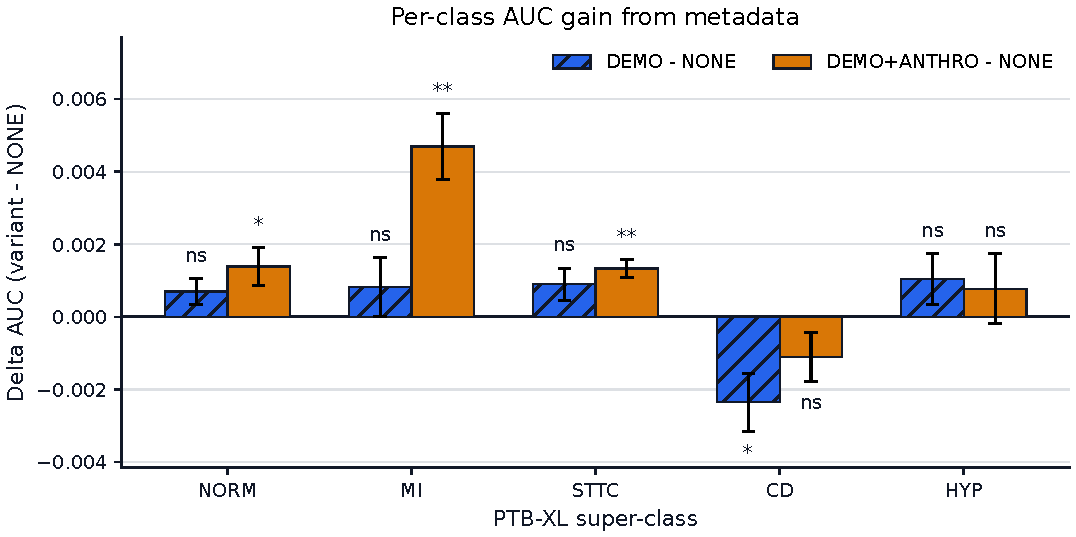
\includegraphics[width=\linewidth]{figures/fig3_per_class_delta_auc.pdf}
\caption{Per-class $\Delta$-AUC of \texttt{demo} and \texttt{demo+anthro} relative to \texttt{none}, mean $\pm$ paired standard error of the mean (SEM) across 10 seeds. Figure annotations indicate raw paired Wilcoxon levels; after BH-FDR correction, only the \texttt{demo+anthro} gains for MI and STTC remain significant. HYP shows no significant effect despite the expectation suggested by voltage-based LVH criteria.}
\label{fig:delta}
\end{figure}

\begin{figure}[H]
\centering
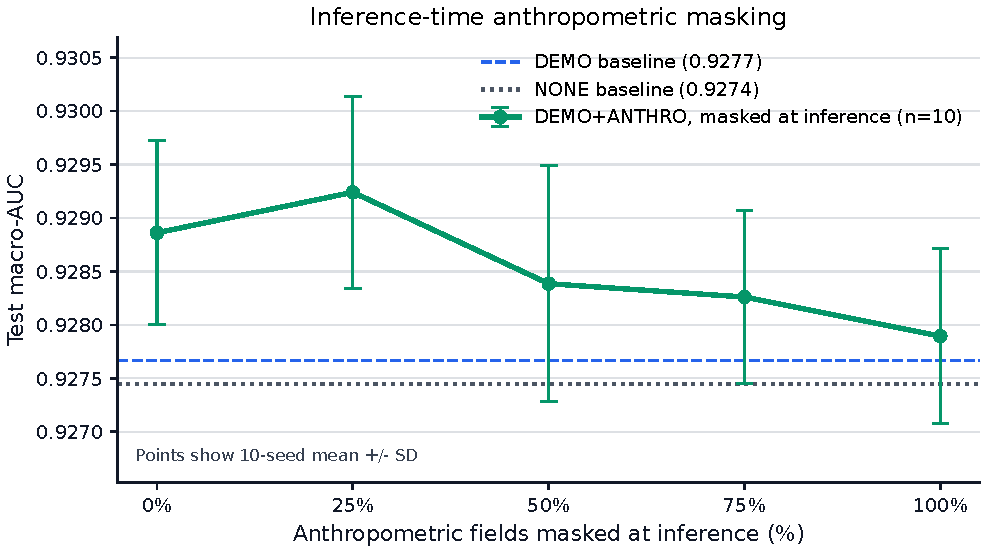
\includegraphics[width=0.95\linewidth]{figures/fig4_missingness_robustness.pdf}
\caption{Missingness robustness of quality-gated fusion. Test macro-AUC as a function of the fraction $\rho$ of anthropometric fields withheld at inference, with consistent updating of the availability mask. Stress-test points remain within a narrow band: $0.9289$ at $\rho{=}0$ (95\% seed-level bootstrap CI $[0.9284, 0.9294]$), $0.9292$ at $\rho{=}0.25$ ($[0.9287, 0.9298]$), $0.9284$ at $\rho{=}0.50$ ($[0.9277, 0.9290]$), $0.9283$ at $\rho{=}0.75$ ($[0.9278, 0.9287]$), and $0.9279$ at $\rho{=}1.0$ ($[0.9274, 0.9284]$). Full anthropometric masking costs $0.0010$ macro-AUC relative to the unmasked model and remains above both the \texttt{demo} baseline ($0.9277$) and the \texttt{none} floor ($0.9274$).}
\label{fig:missing}
\end{figure}

\begin{figure}[H]
\centering
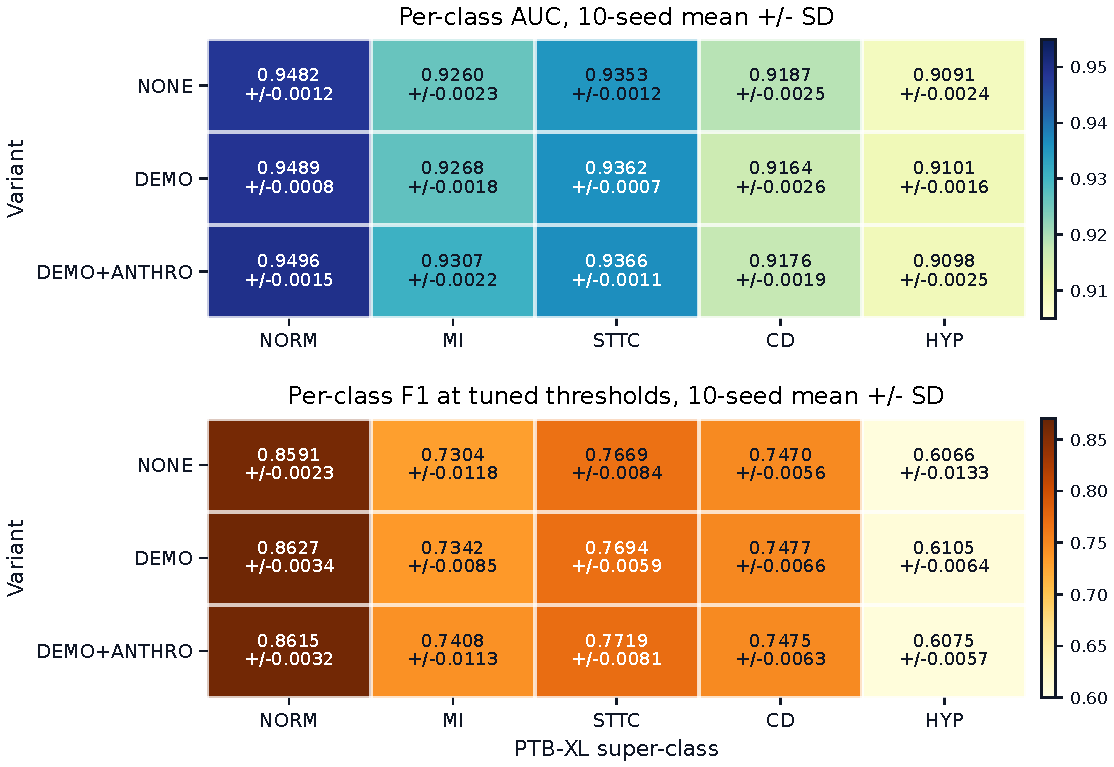
\includegraphics[width=\linewidth]{figures/fig5_per_class_heatmap.pdf}
\caption{Per-class AUC (top, sequential YlGnBu scale) and best-threshold $F_1$ (bottom, sequential YlOrBr scale) for the three ablation variants, mean $\pm$ standard deviation across 10 seeds. Colour intensity visualises absolute performance and descriptive changes between variants; the printed cell values give the exact mean $\pm$ standard deviation, AUC shifts are largest in the MI column, and $F_1$ changes are small and should be read descriptively.}
\label{fig:heat}
\end{figure}

\begin{figure}[H]
\centering

\includegraphics[width=\linewidth]{figures/fig6_fused_vs_ecg_gap.pdf}
\caption{Seed-level gap $\mathrm{AUC}_{\mathrm{fused}} - \mathrm{AUC}_{\mathrm{ecg}}$ on the test fold, where positive values mean that the fused branch outperforms the ECG-only branch. The \texttt{demo+anthro} variant shows a positive gap for every seed (rounded median $+0.0013$), whereas \texttt{none} and \texttt{demo} are centred near zero. This is consistent with the validation-based selection of $w^{\ast}{=}1.0$ for all 30 runs.}
\label{fig:blend}
\end{figure}

% ---- Bibliography -----------------------------------------
\reftitle{References}
\externalbibliography{yes}
\bibliography{bibliography}

\end{document}
